\chapter{Technische Zeichnungen}

\begin{figure}[ht!]
	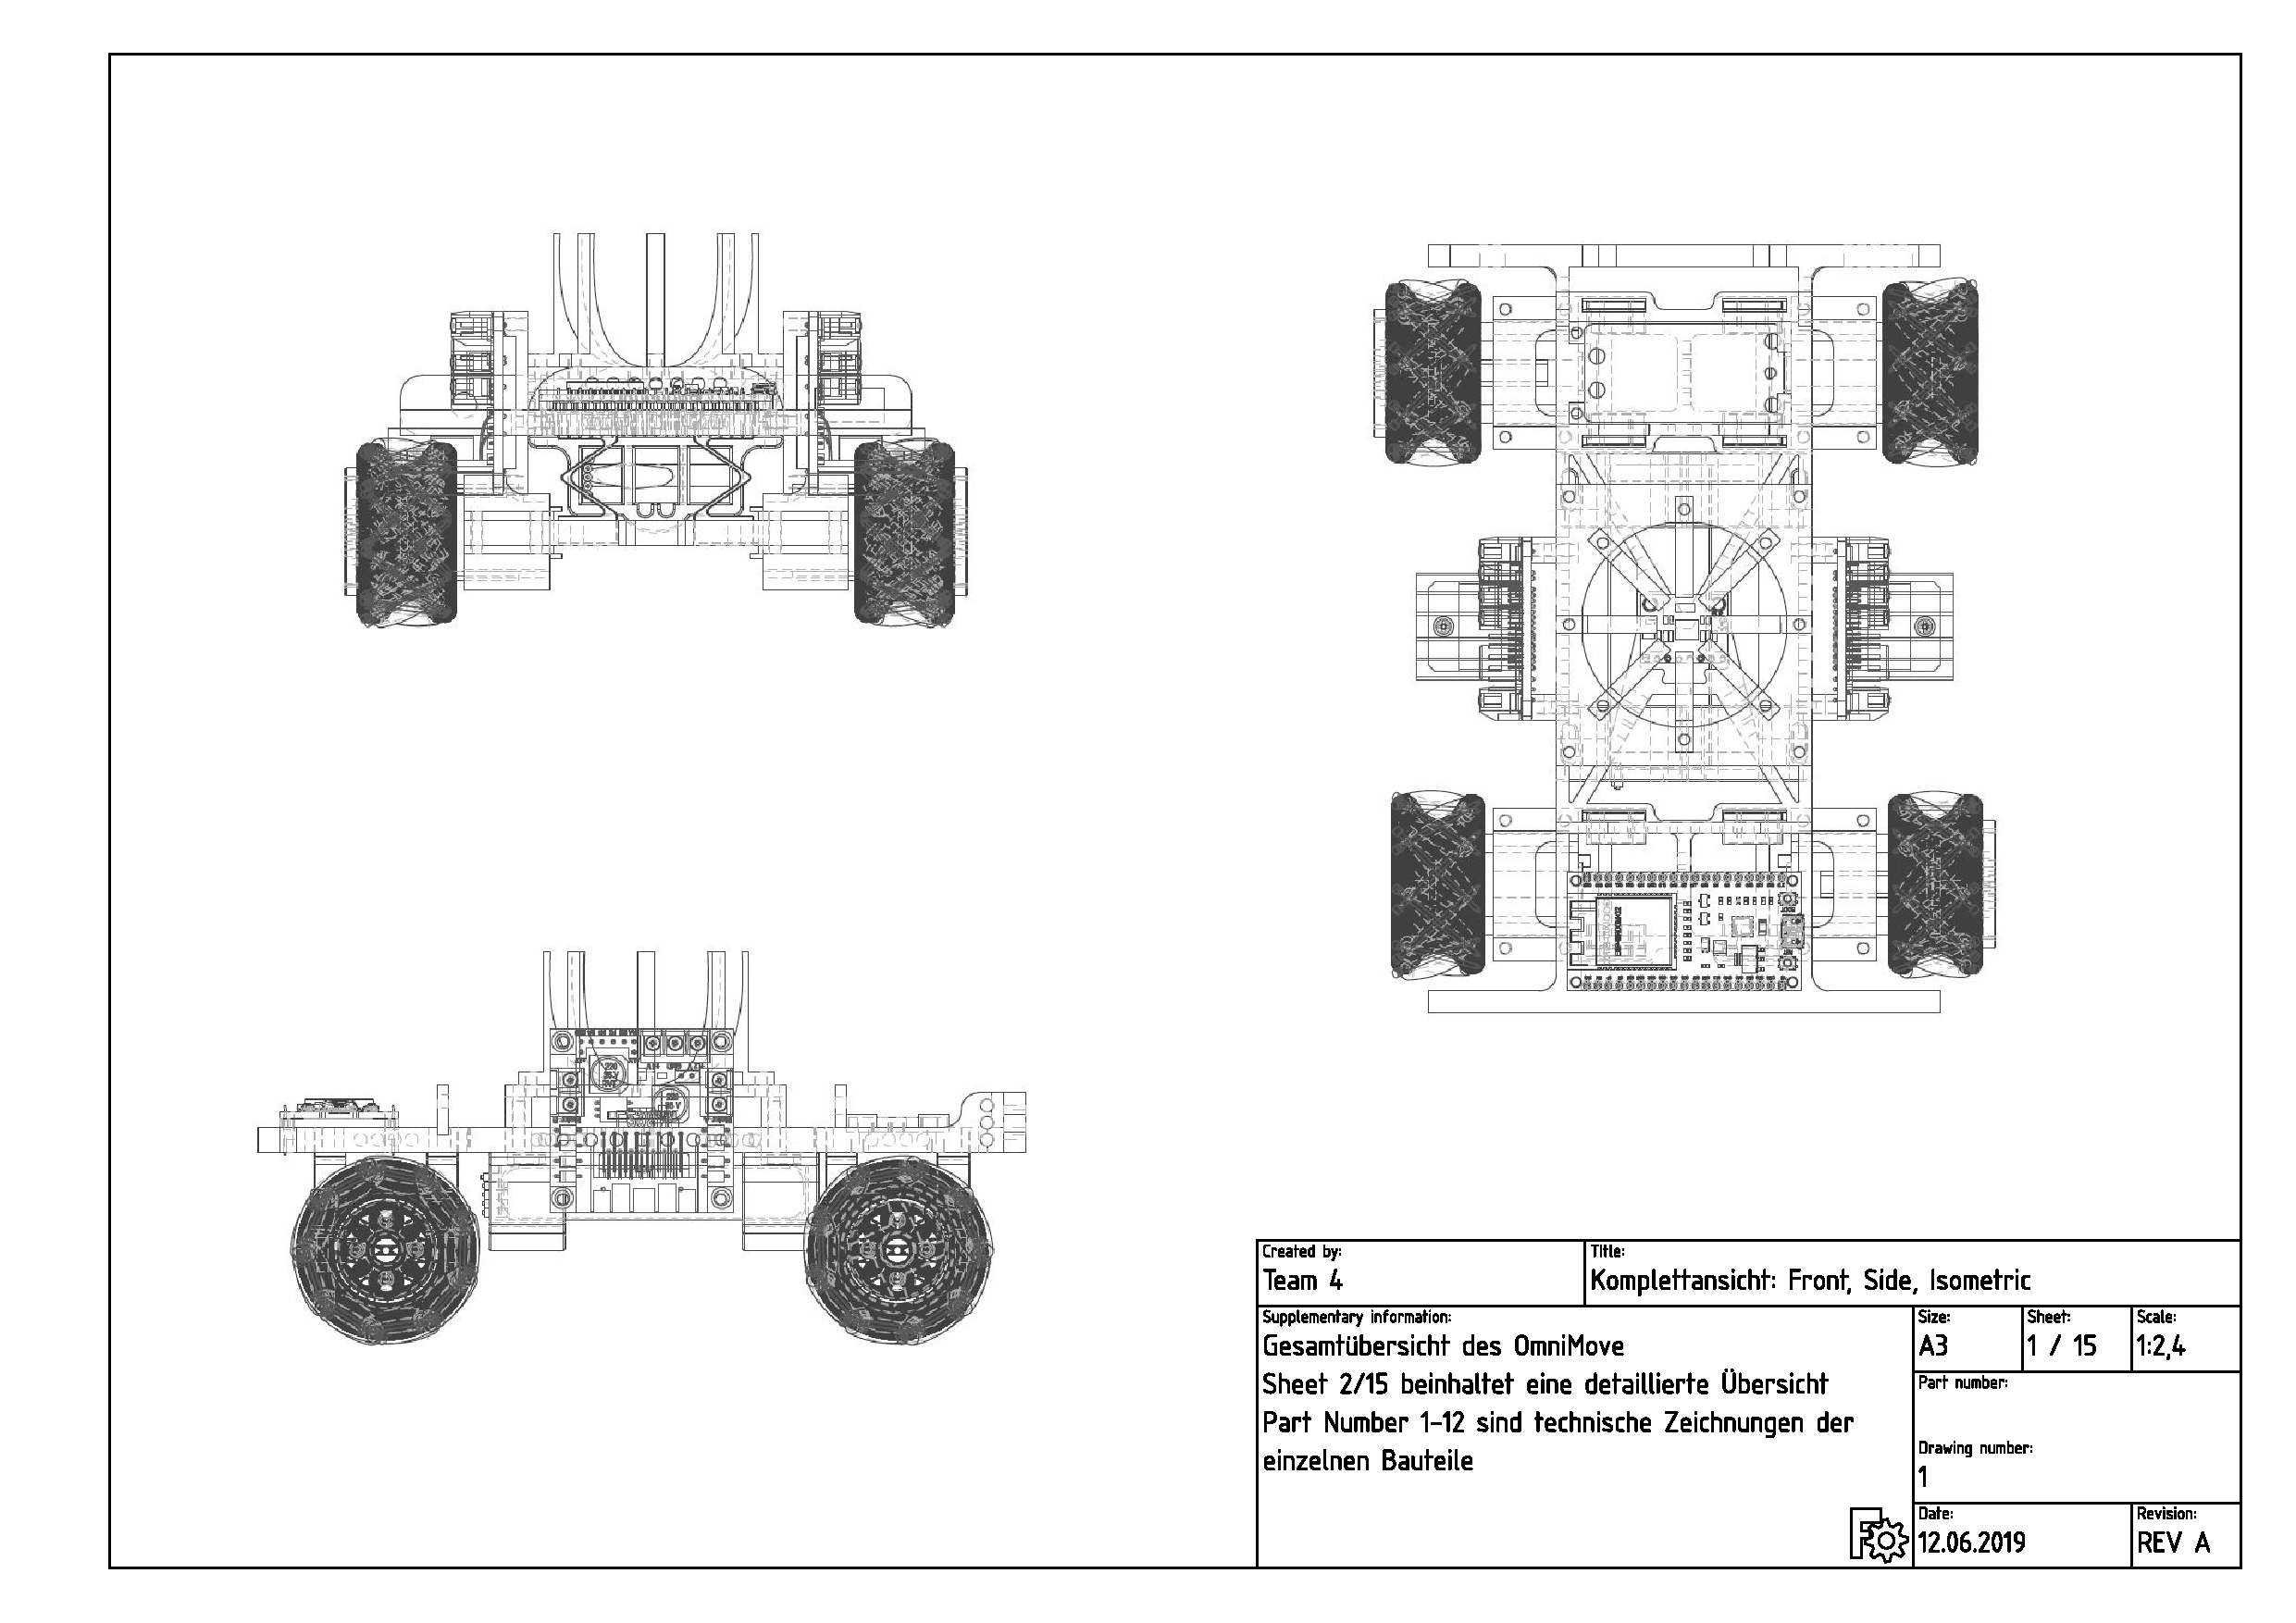
\includegraphics[width=\textwidth]{../techzeich/00.PDF} 	
	\caption{Komplettansicht}
\end{figure}

\begin{figure}[ht!]
	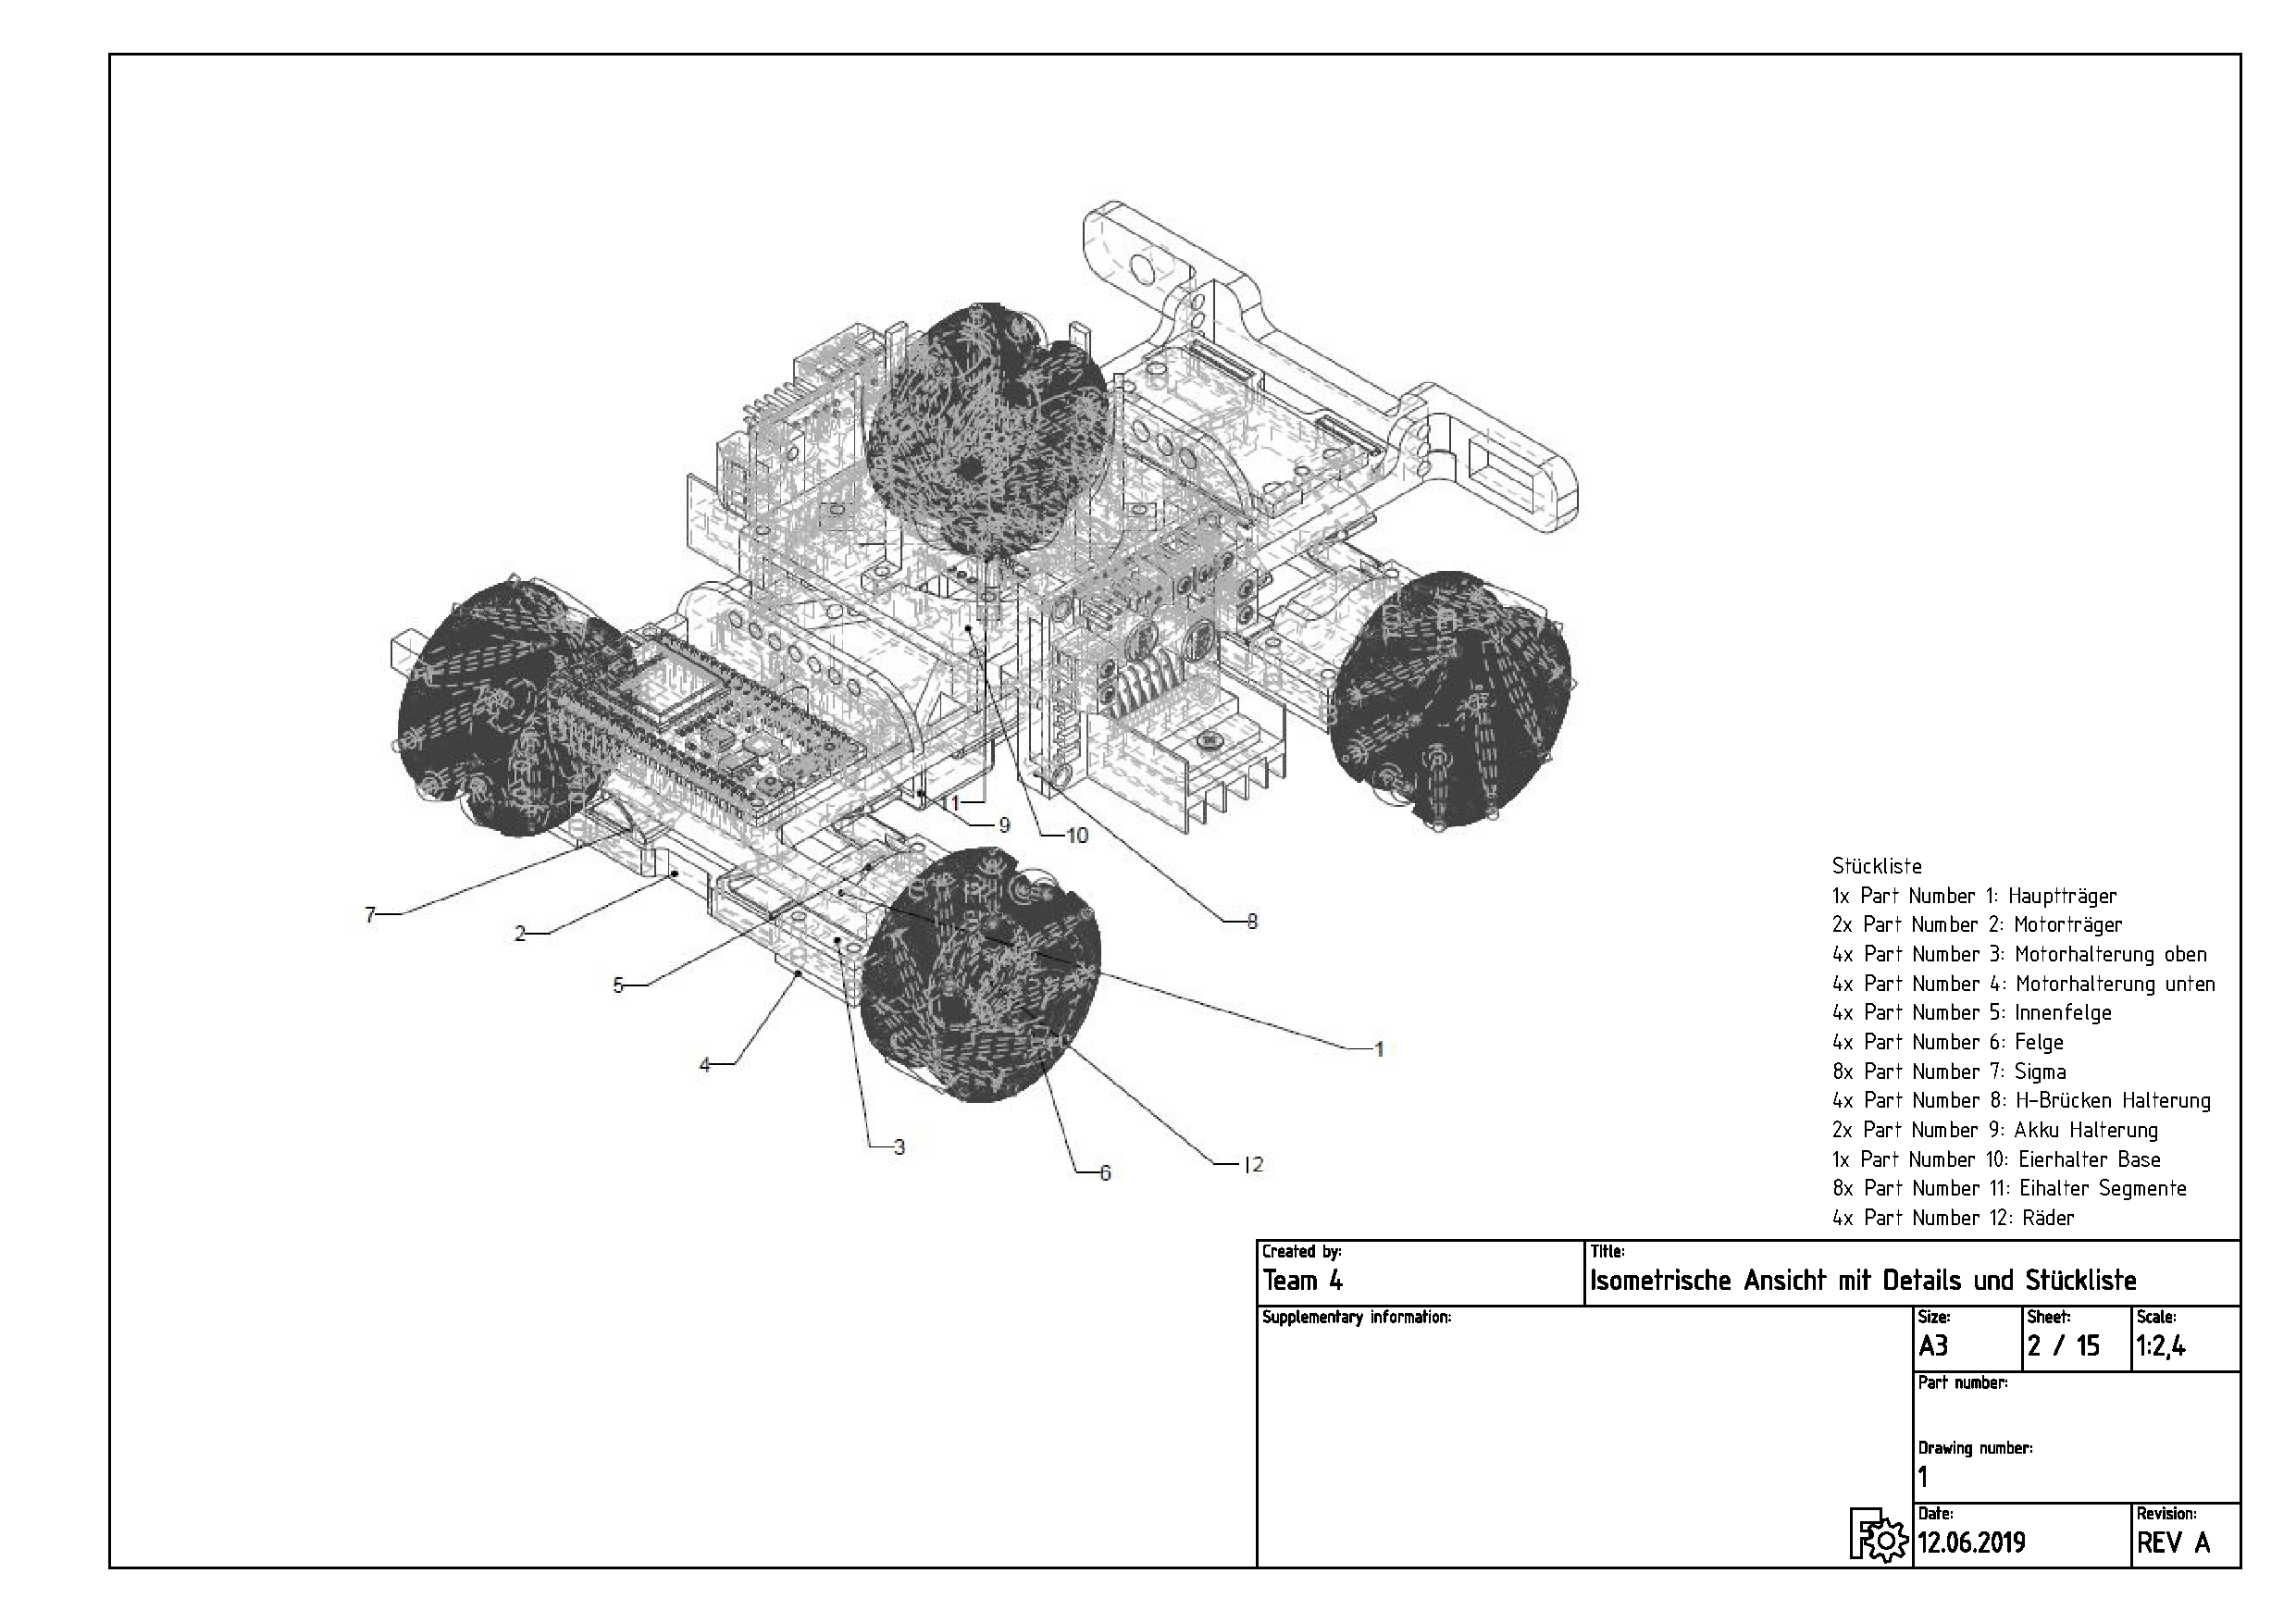
\includegraphics[width=\textwidth]{../techzeich/01.PDF} 
	\caption{Isometrisch und St�ckliste}
\end{figure}

\begin{figure}[ht!]
	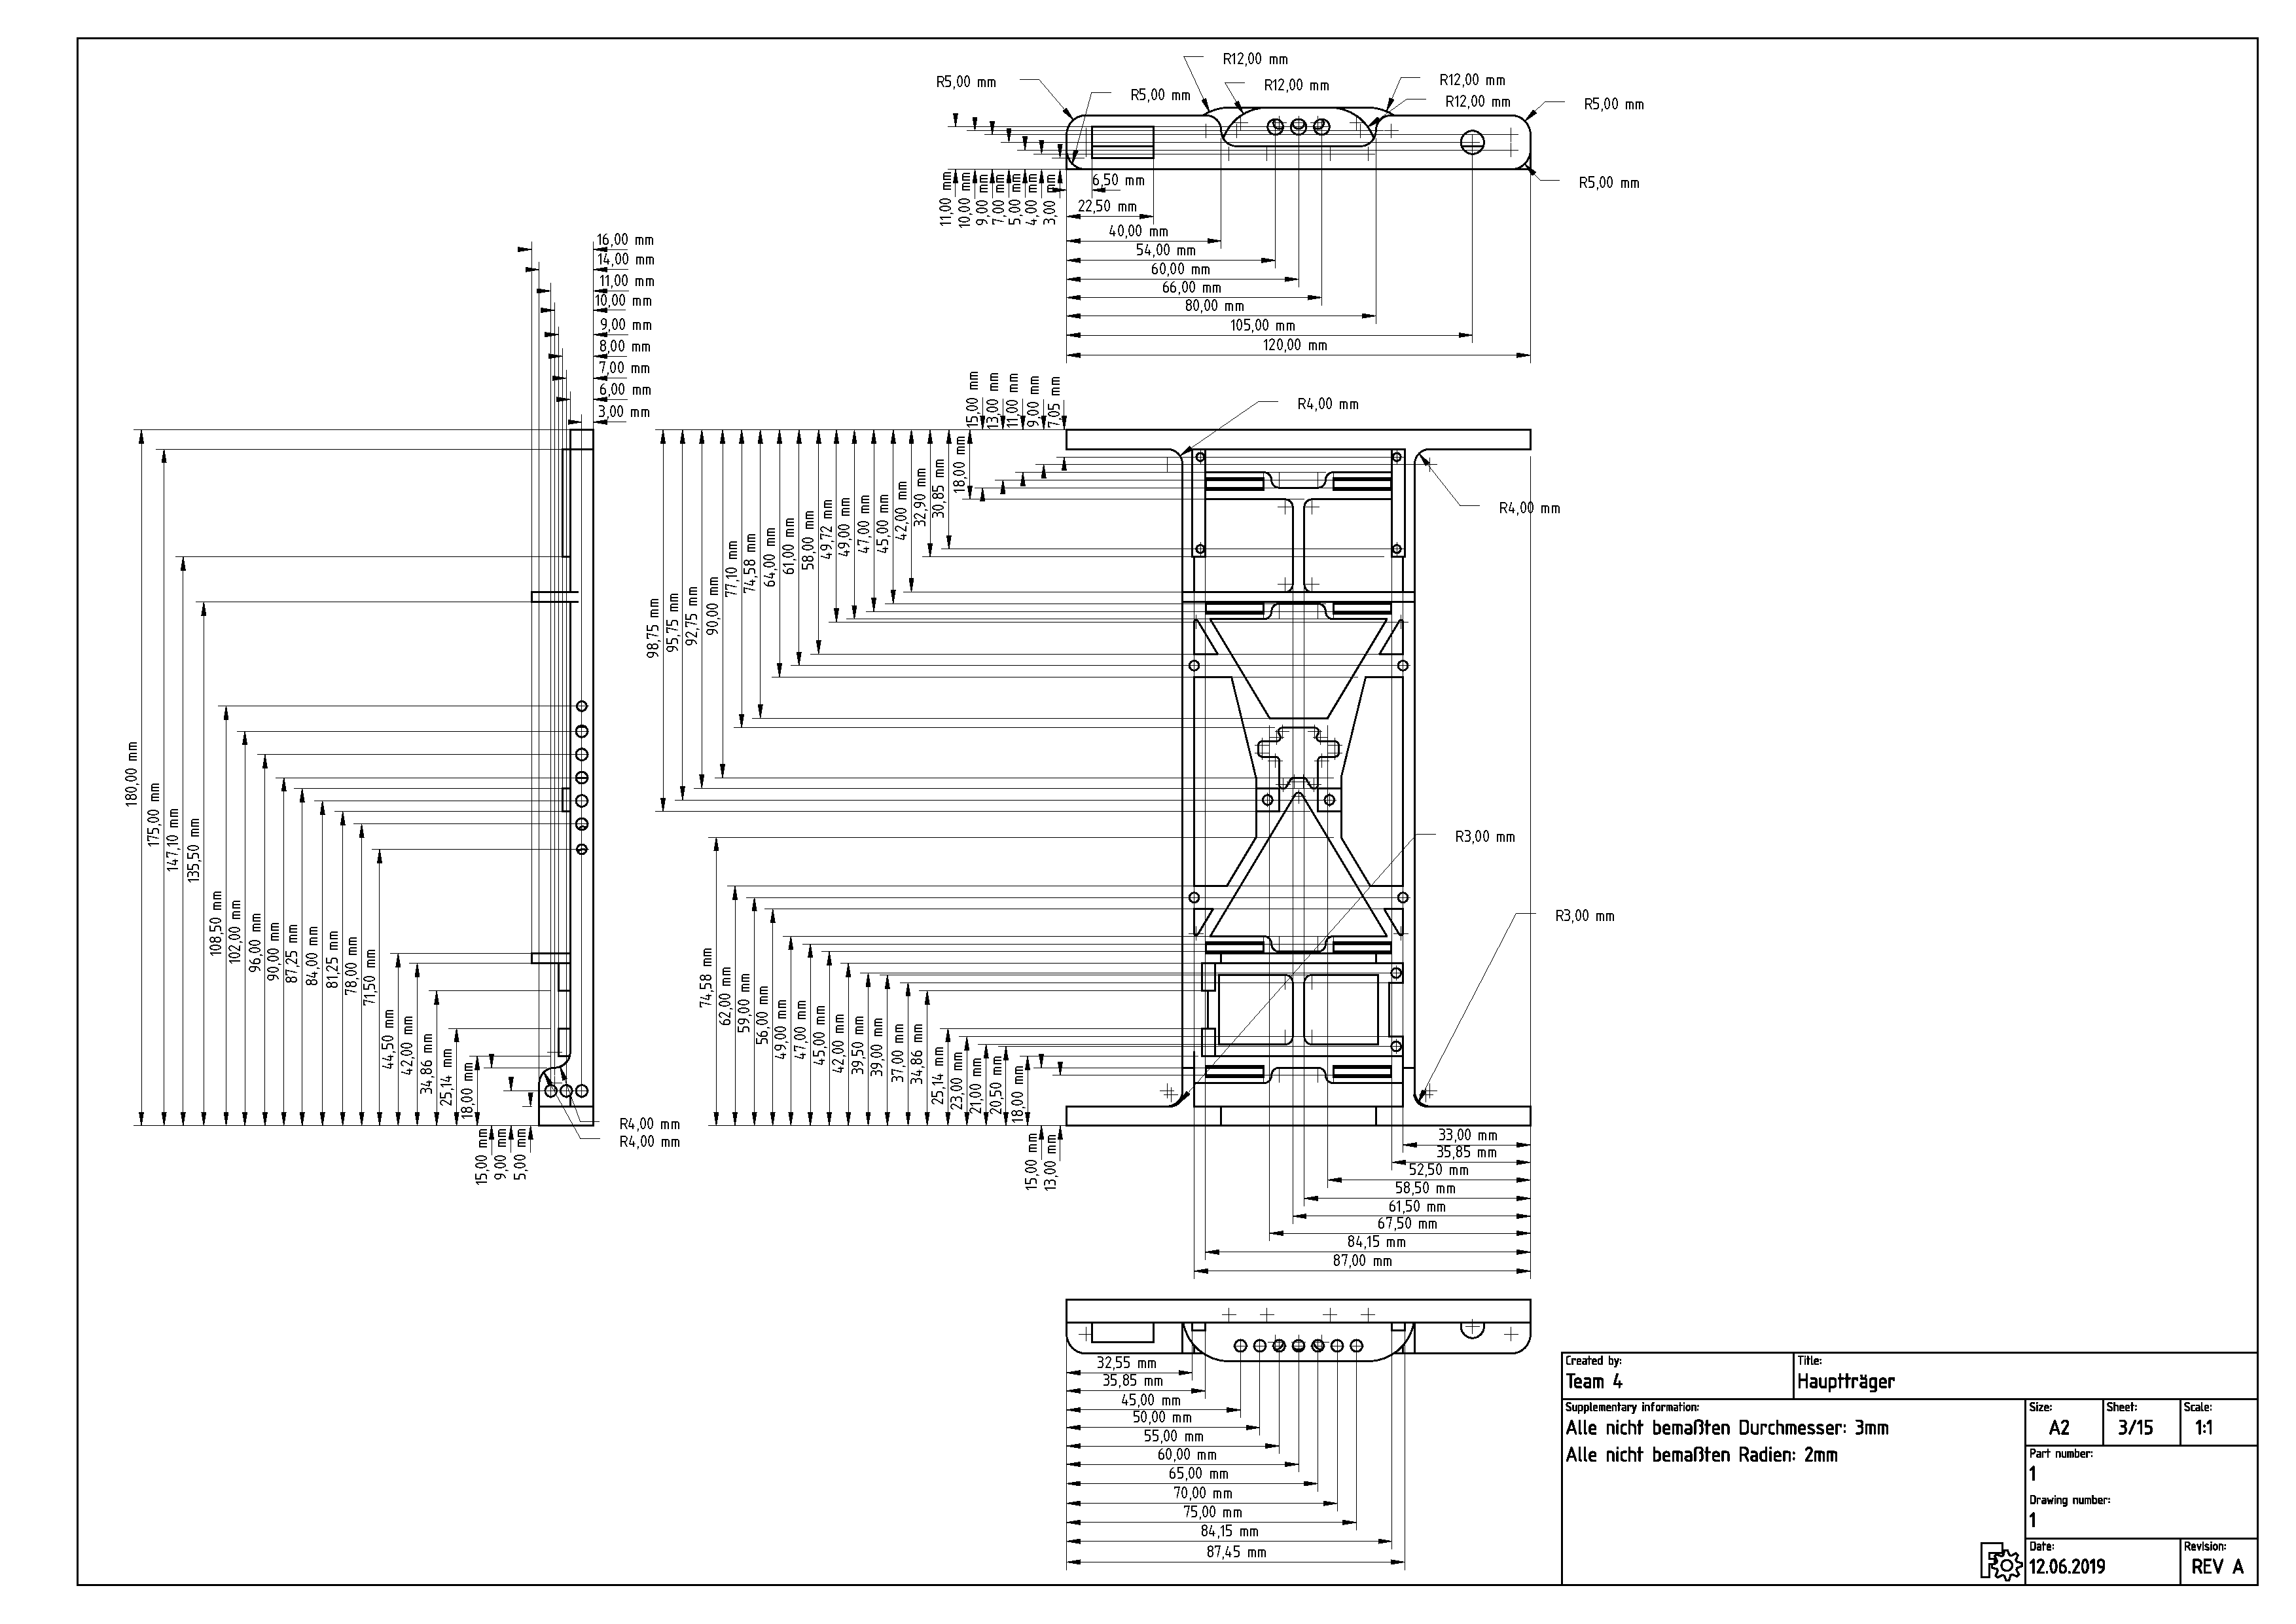
\includegraphics[width=\textwidth]{../techzeich/1.PDF} 	
	\caption{Haupttr�ger}
\end{figure}

\begin{figure}[ht!]
	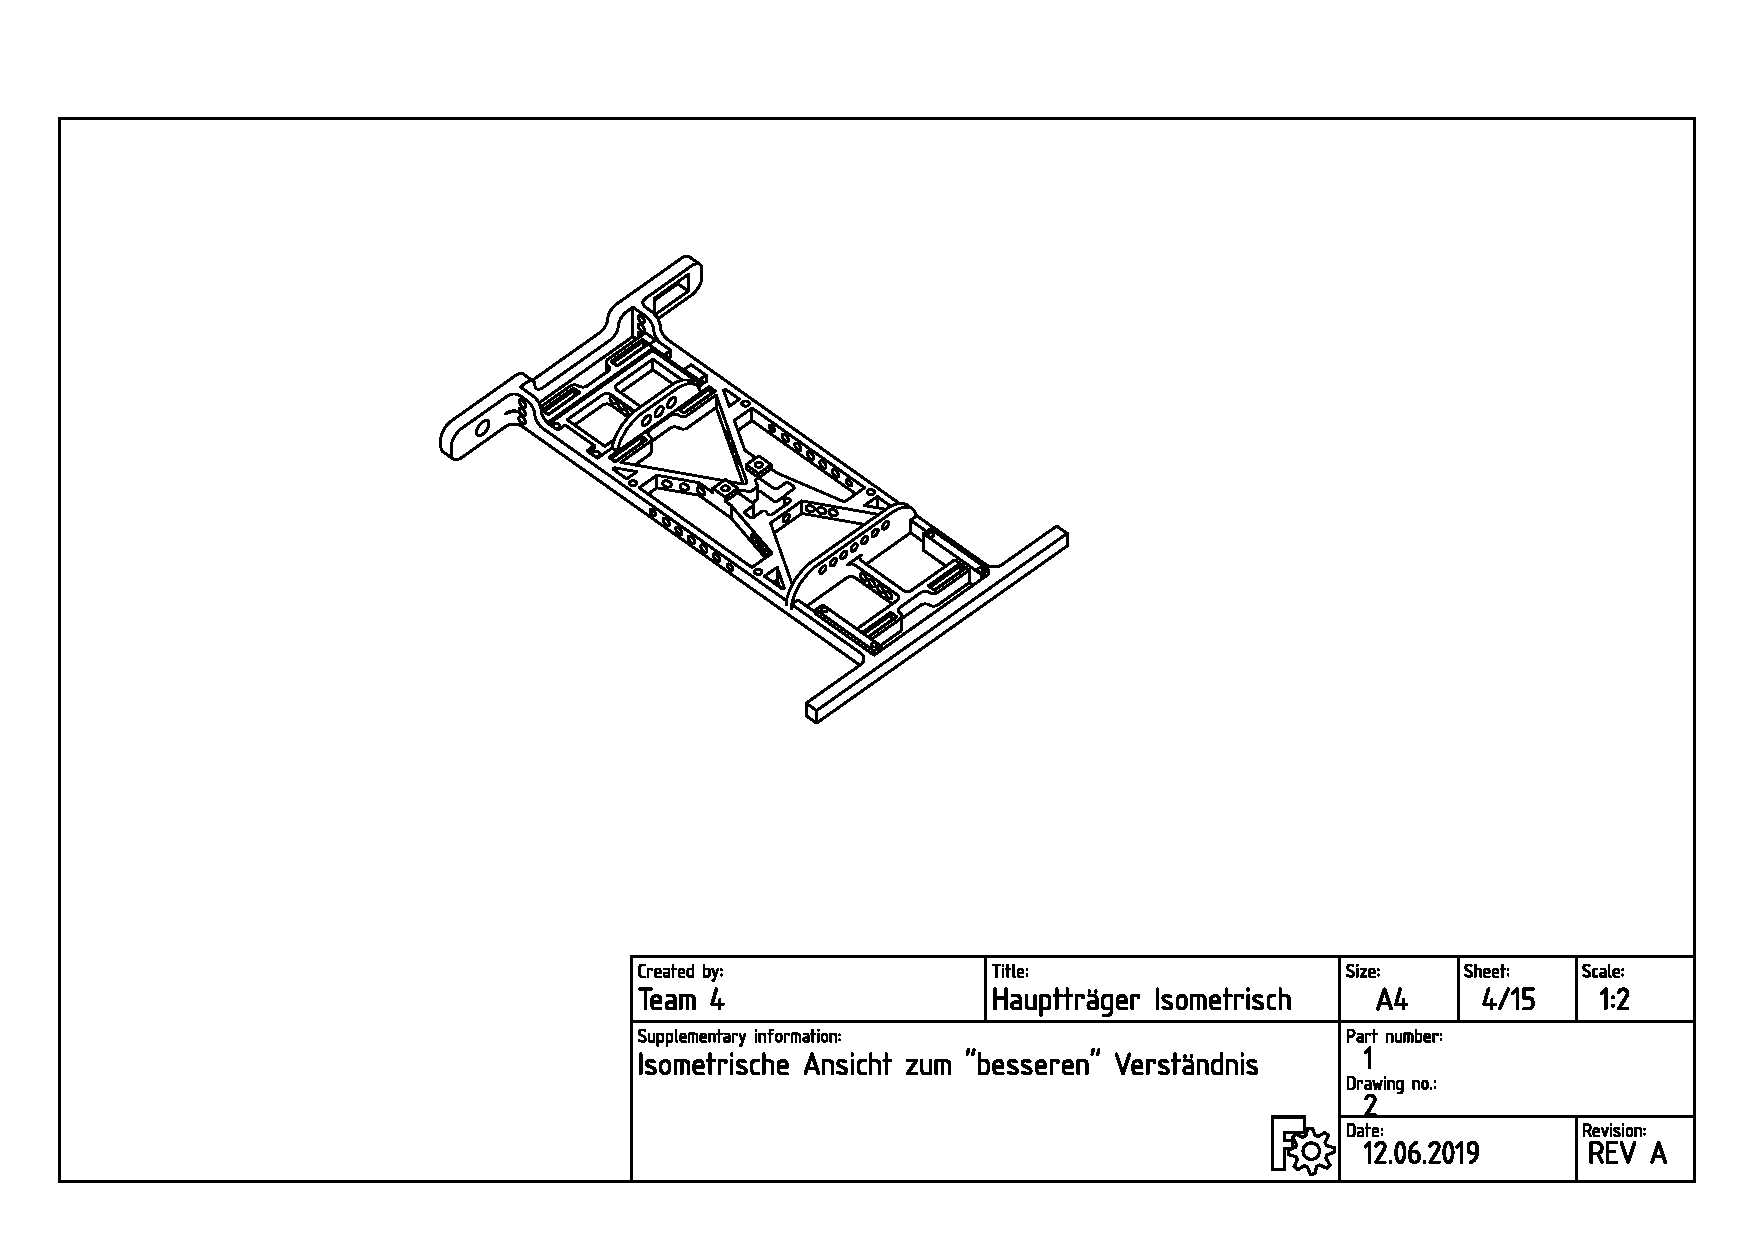
\includegraphics[width=\textwidth]{../techzeich/1iso.PDF} 	
	\caption{Haupttr�ger Isometrisch}
\end{figure}

\begin{figure}[ht!]
	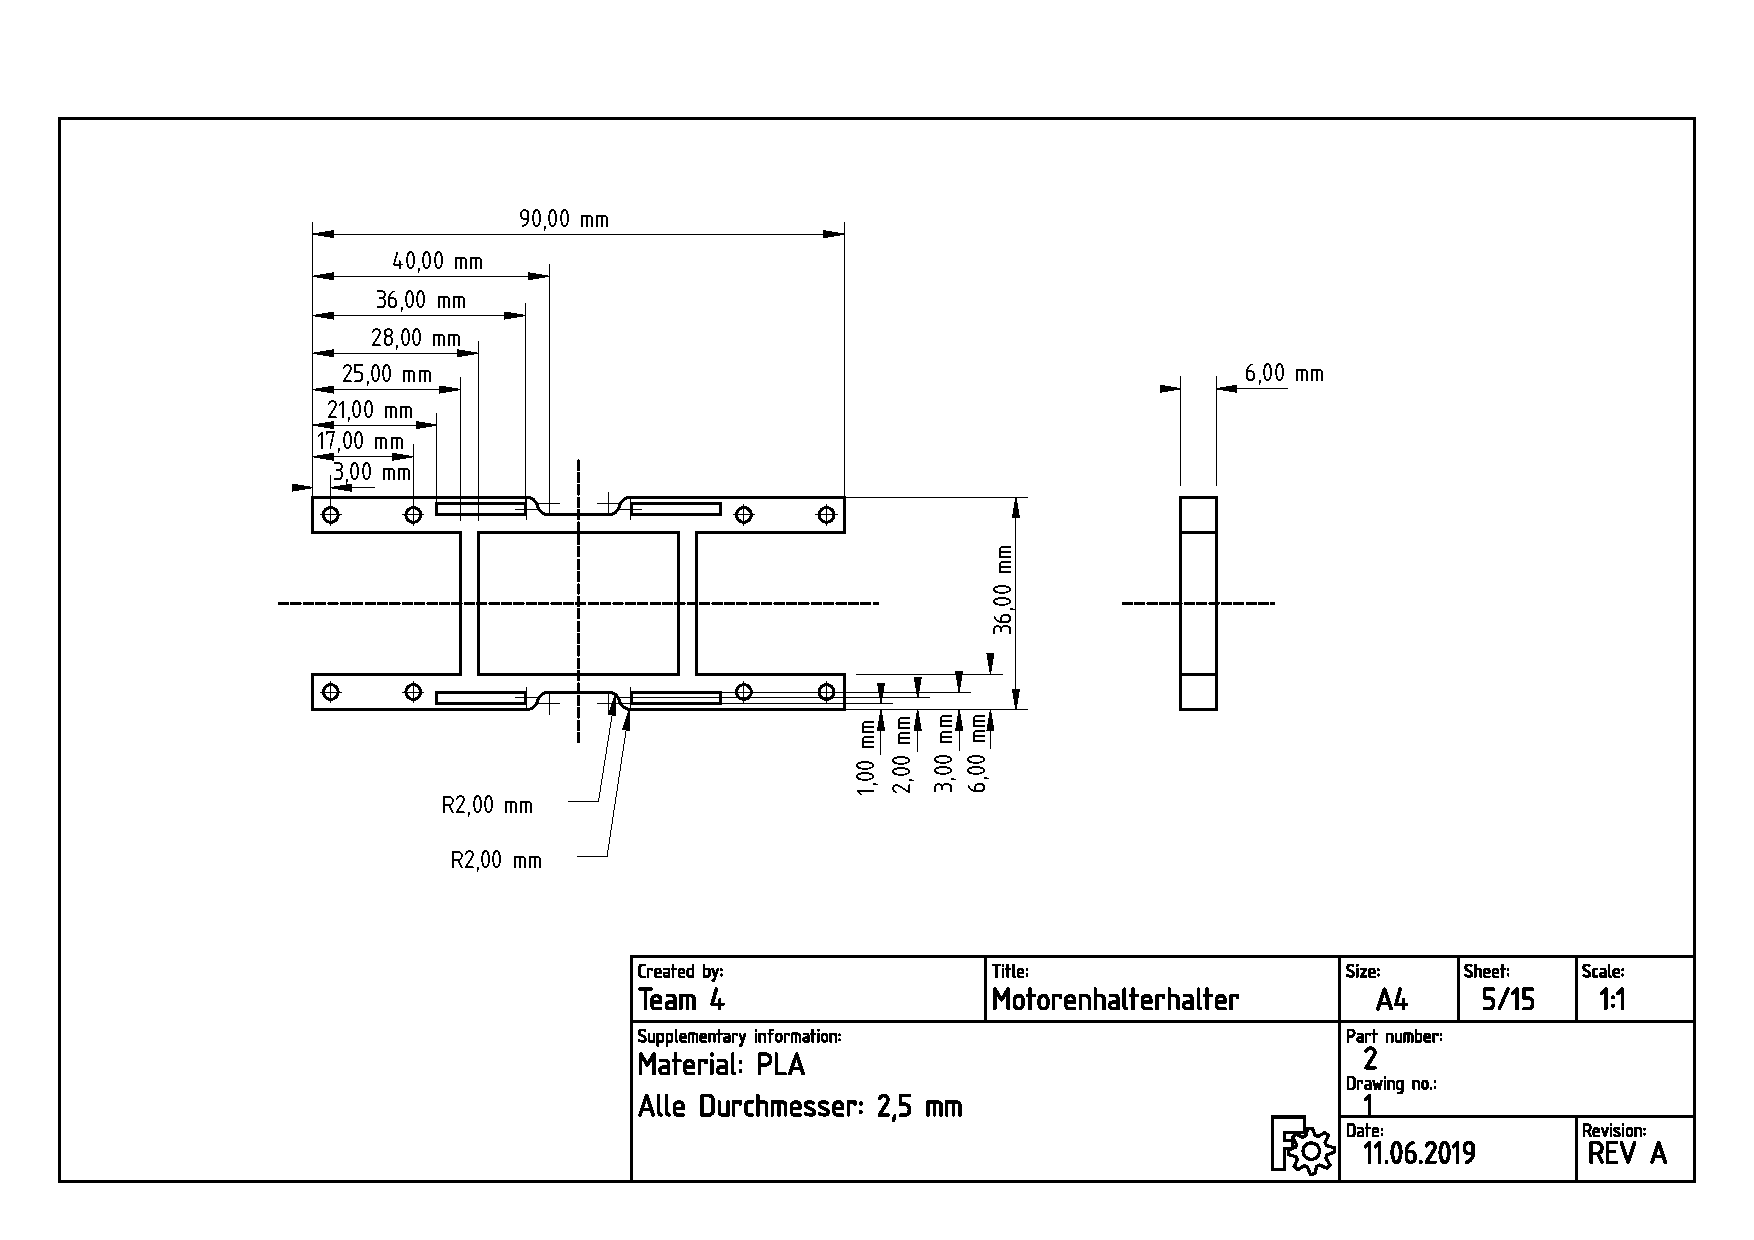
\includegraphics[width=\textwidth]{../techzeich/2.PDF} 	
	\caption{Motorenhalterhalter}
\end{figure}

\begin{figure}[ht!]
	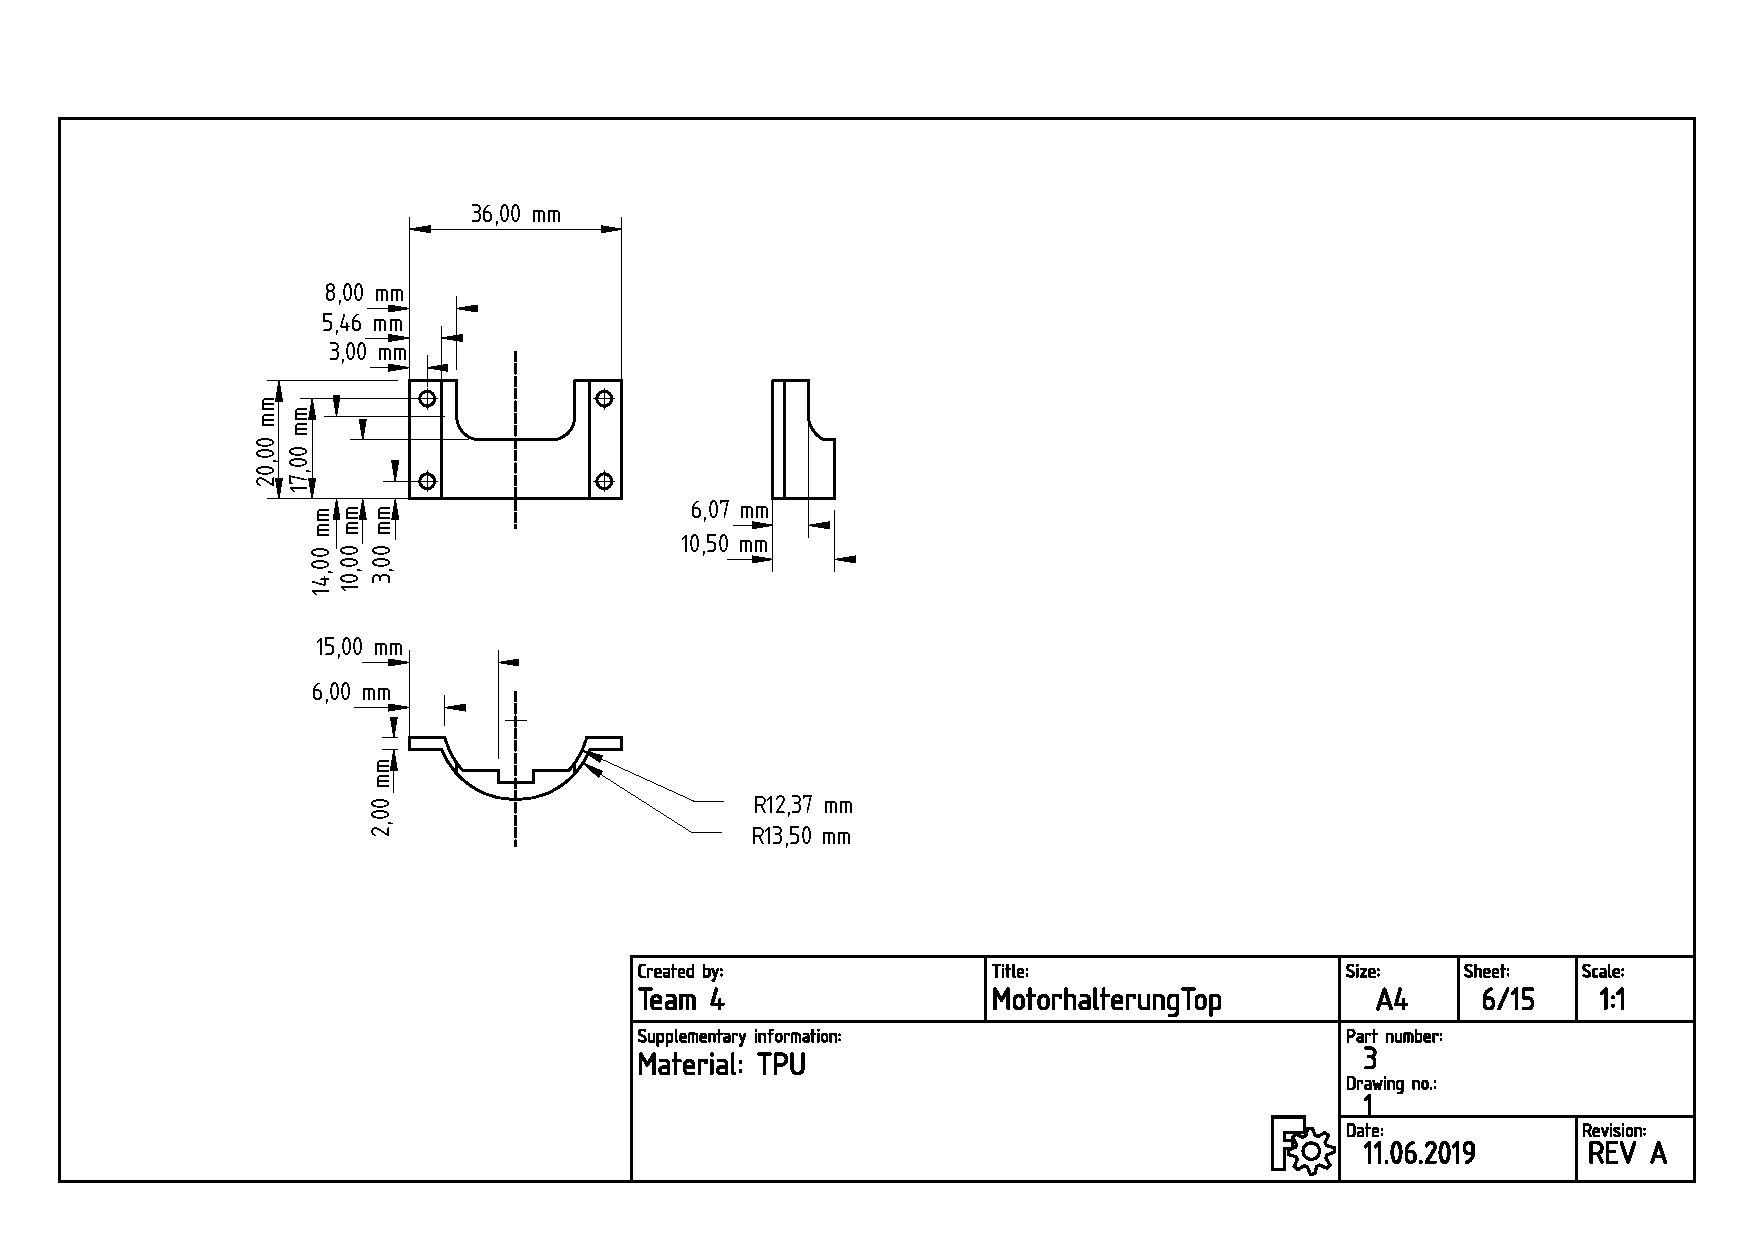
\includegraphics[width=\textwidth]{../techzeich/3.PDF} 	
	\caption{Motorenhalterung Oben}
\end{figure}
\begin{figure}[ht!]
	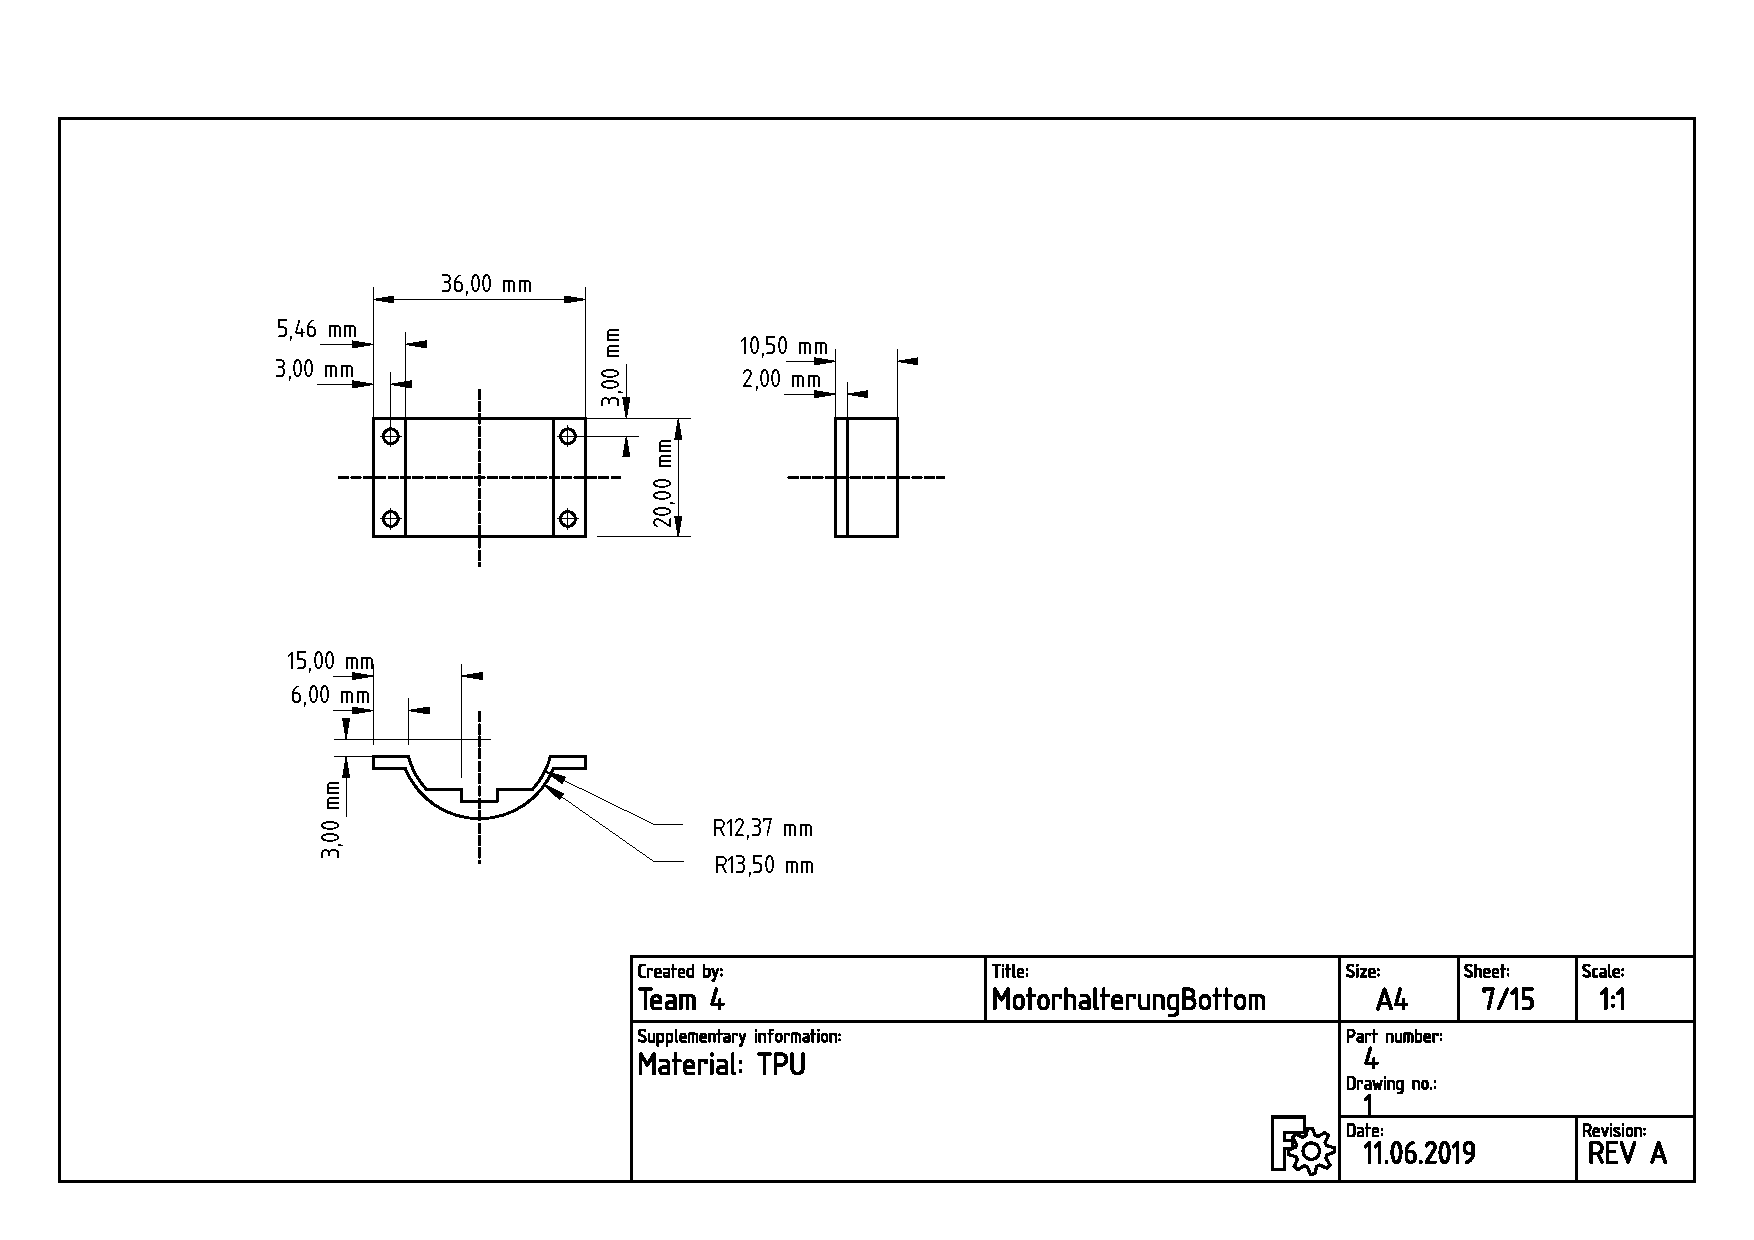
\includegraphics[width=\textwidth]{../techzeich/4.PDF} 	
	\caption{Motorenhalterung Unten}
\end{figure}
\begin{figure}[ht!]
	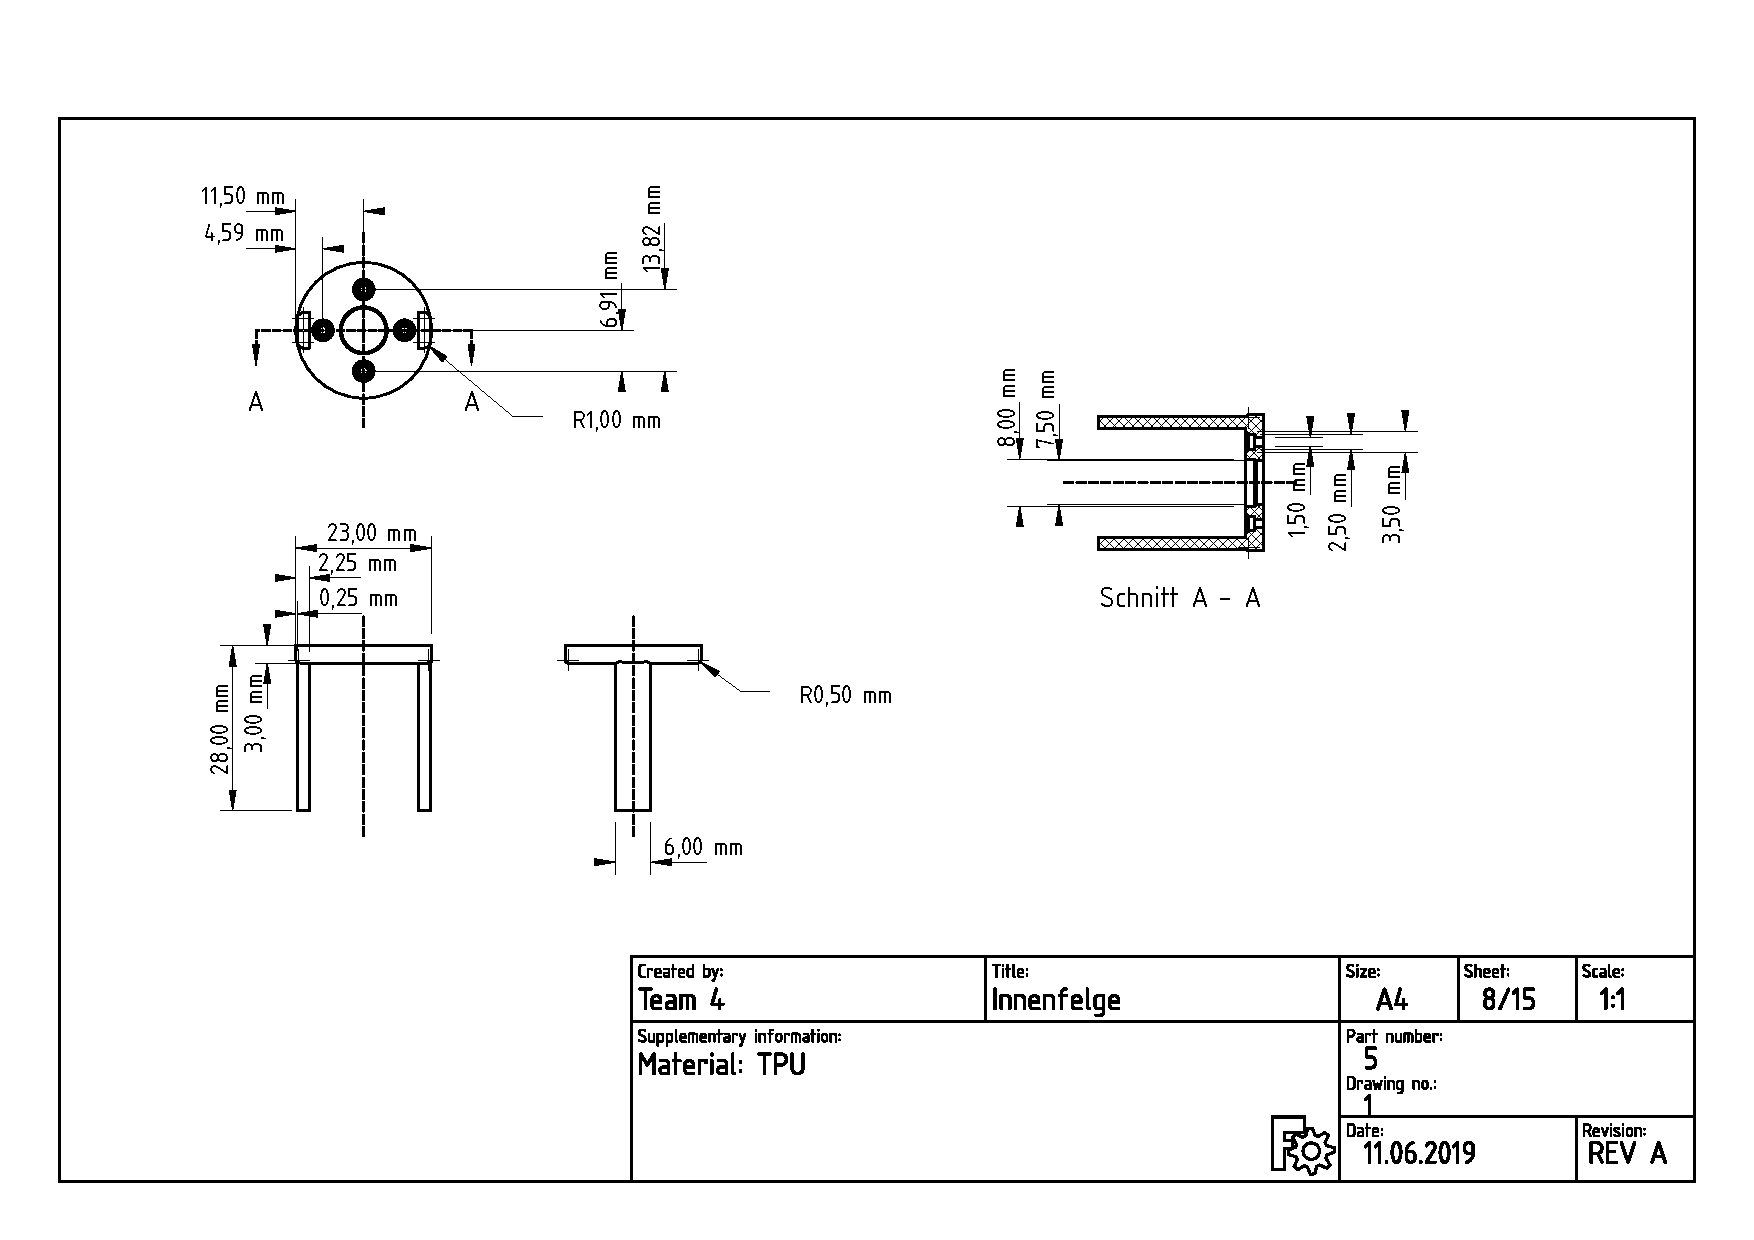
\includegraphics[width=\textwidth]{../techzeich/5.PDF} 	
	\caption{Innenfelge}
\end{figure}
\begin{figure}[ht!]
	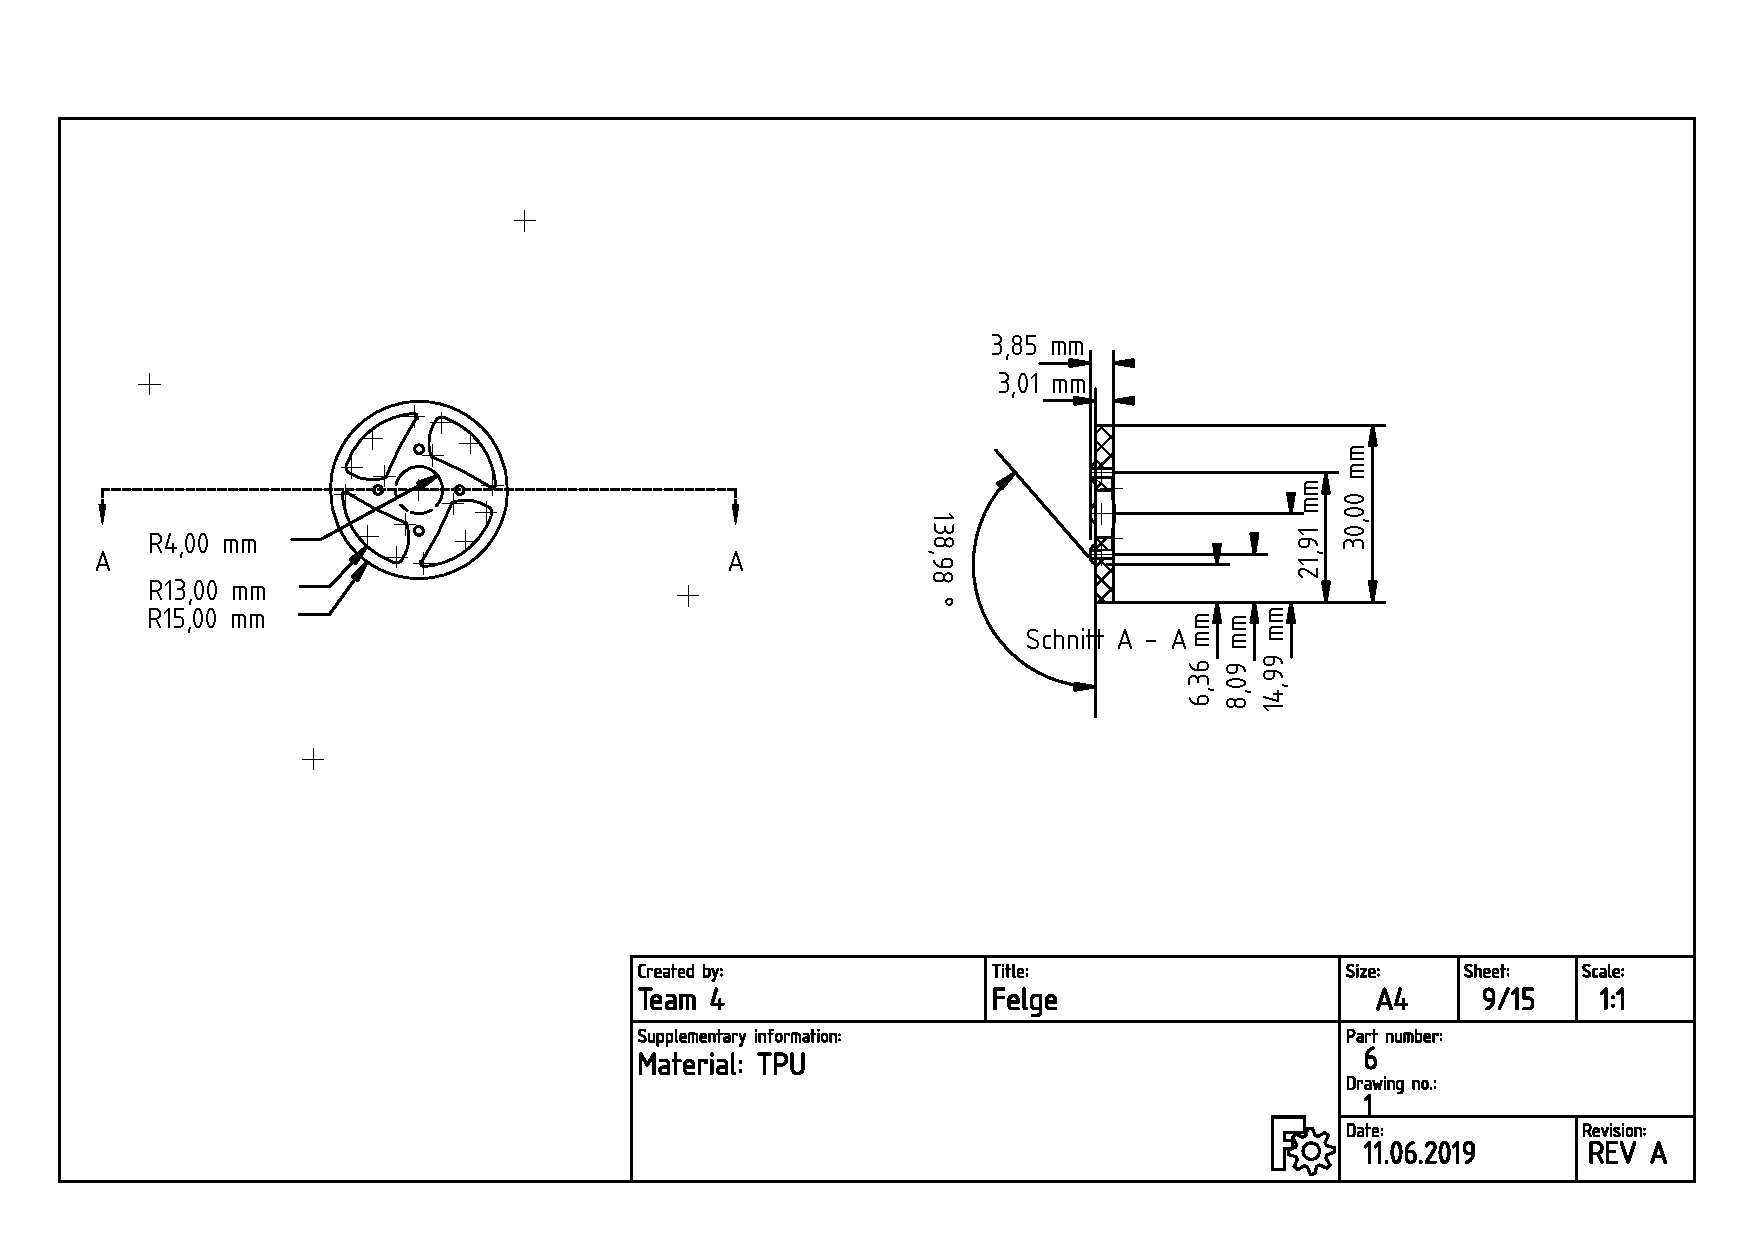
\includegraphics[width=\textwidth]{../techzeich/6.PDF} 	
	\caption{Felge}
\end{figure}
\begin{figure}[ht!]
	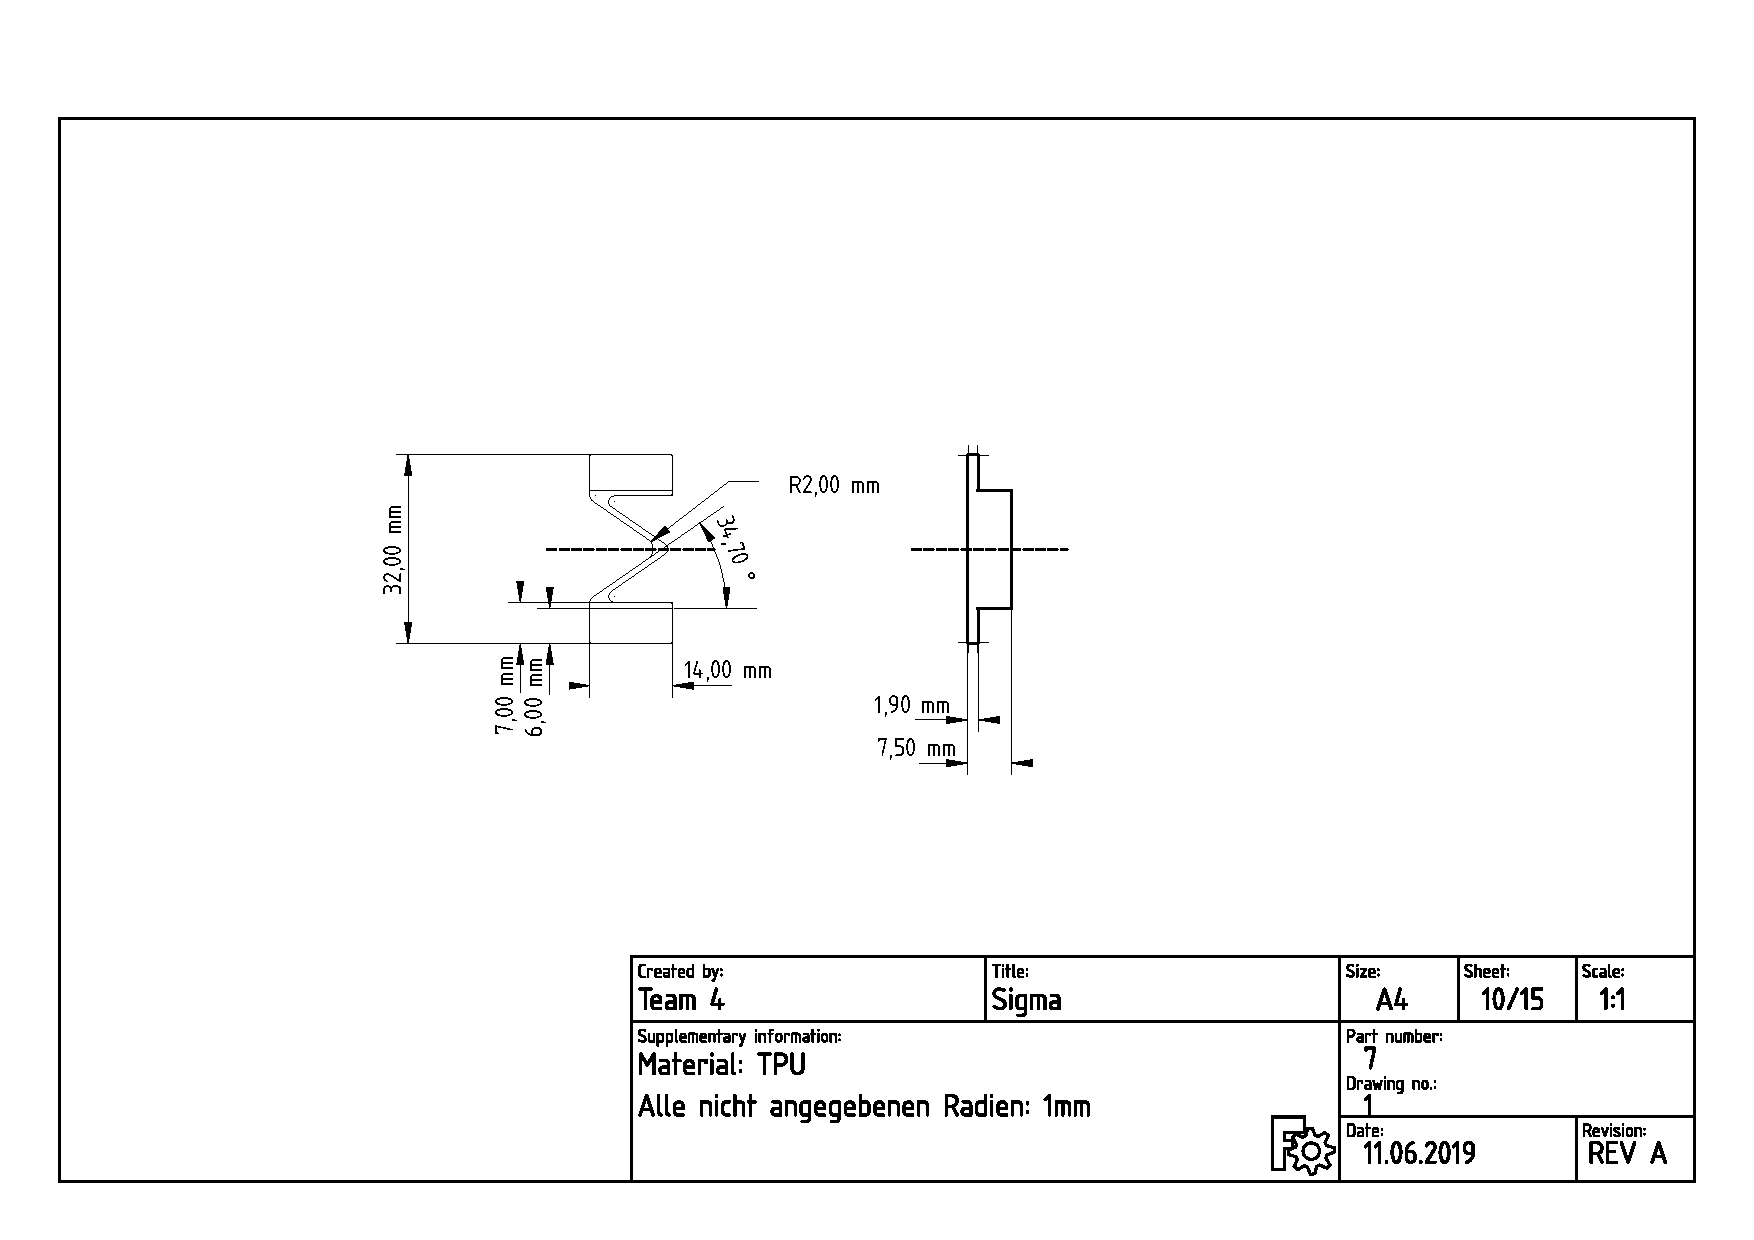
\includegraphics[width=\textwidth]{../techzeich/7.PDF} 	
	\caption{Sigma}
\end{figure}
\begin{figure}[ht!]
	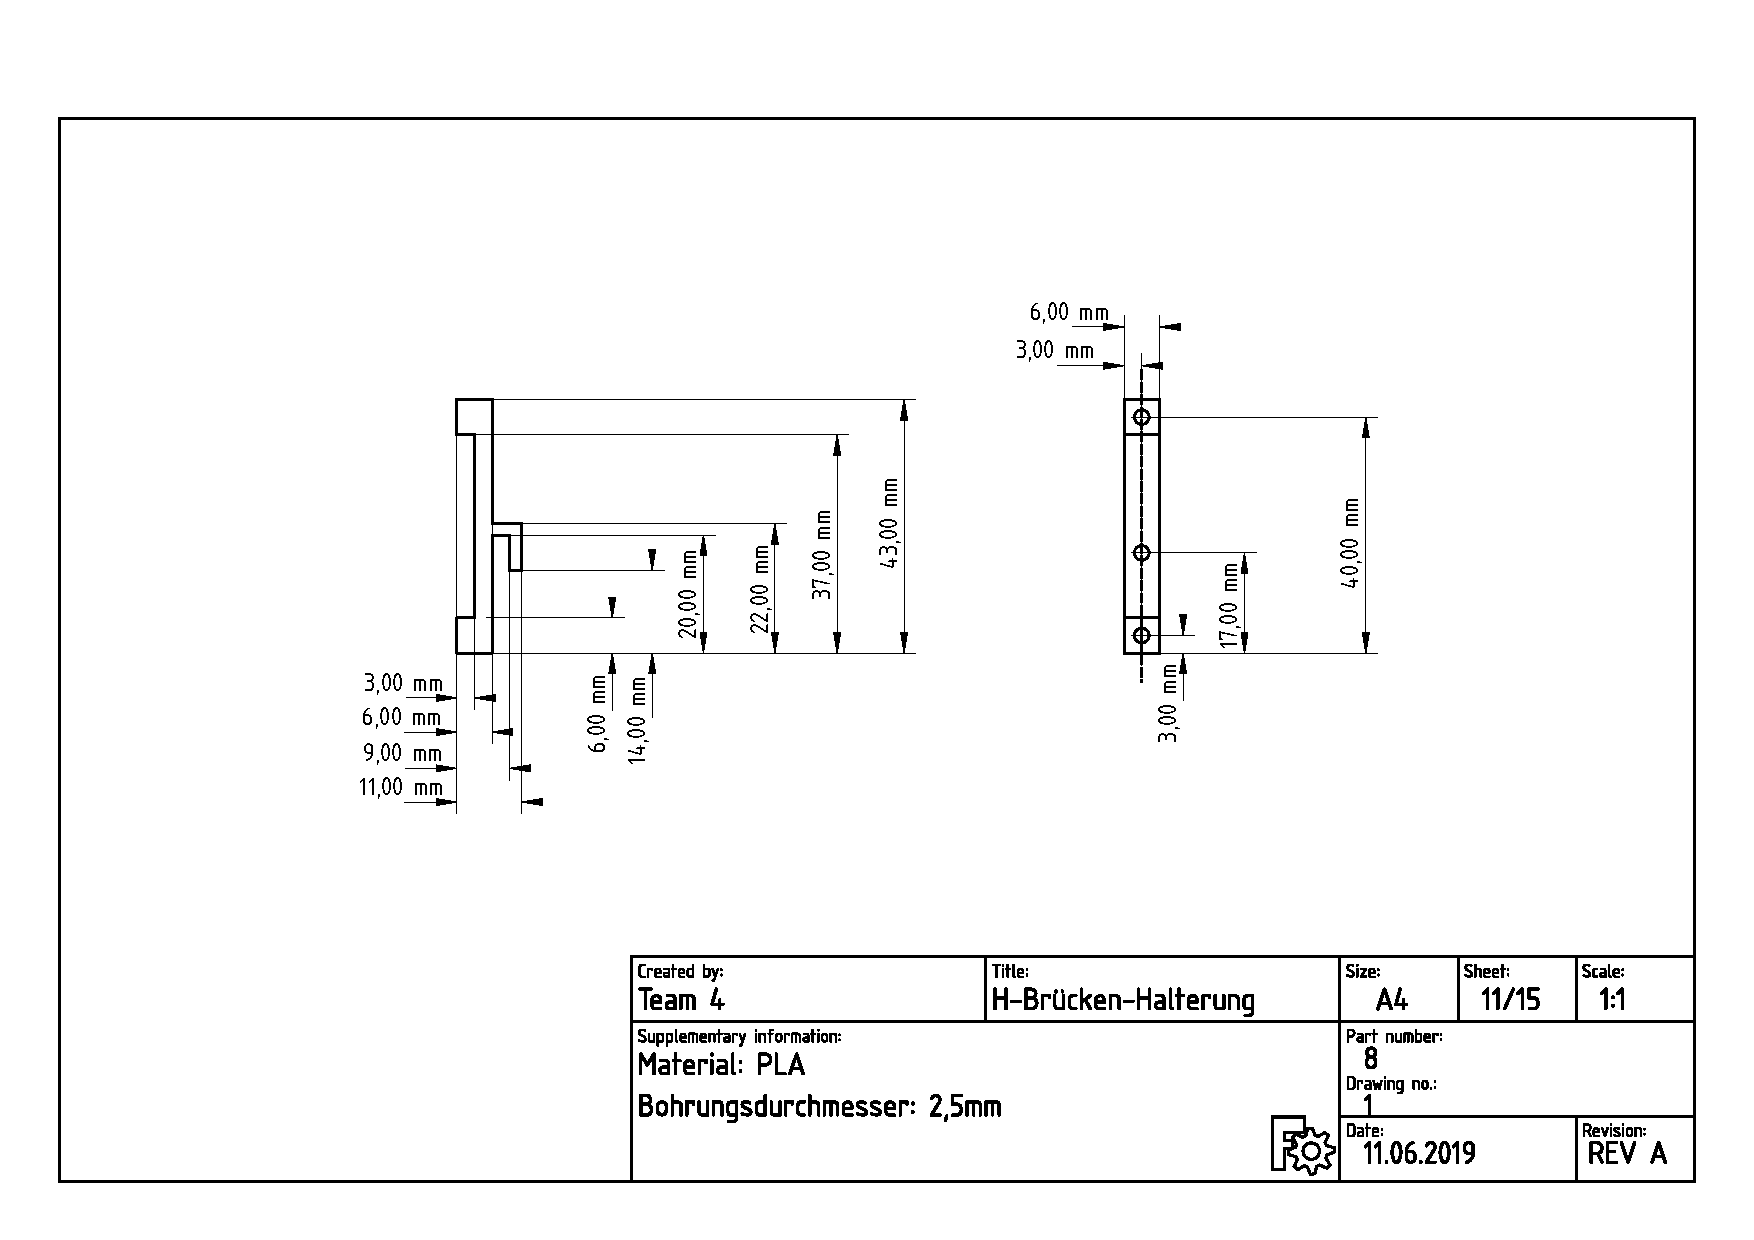
\includegraphics[width=\textwidth]{../techzeich/8.PDF} 	
	\caption{H-Br�cken-Halterung}
\end{figure}
\begin{figure}[ht!]
	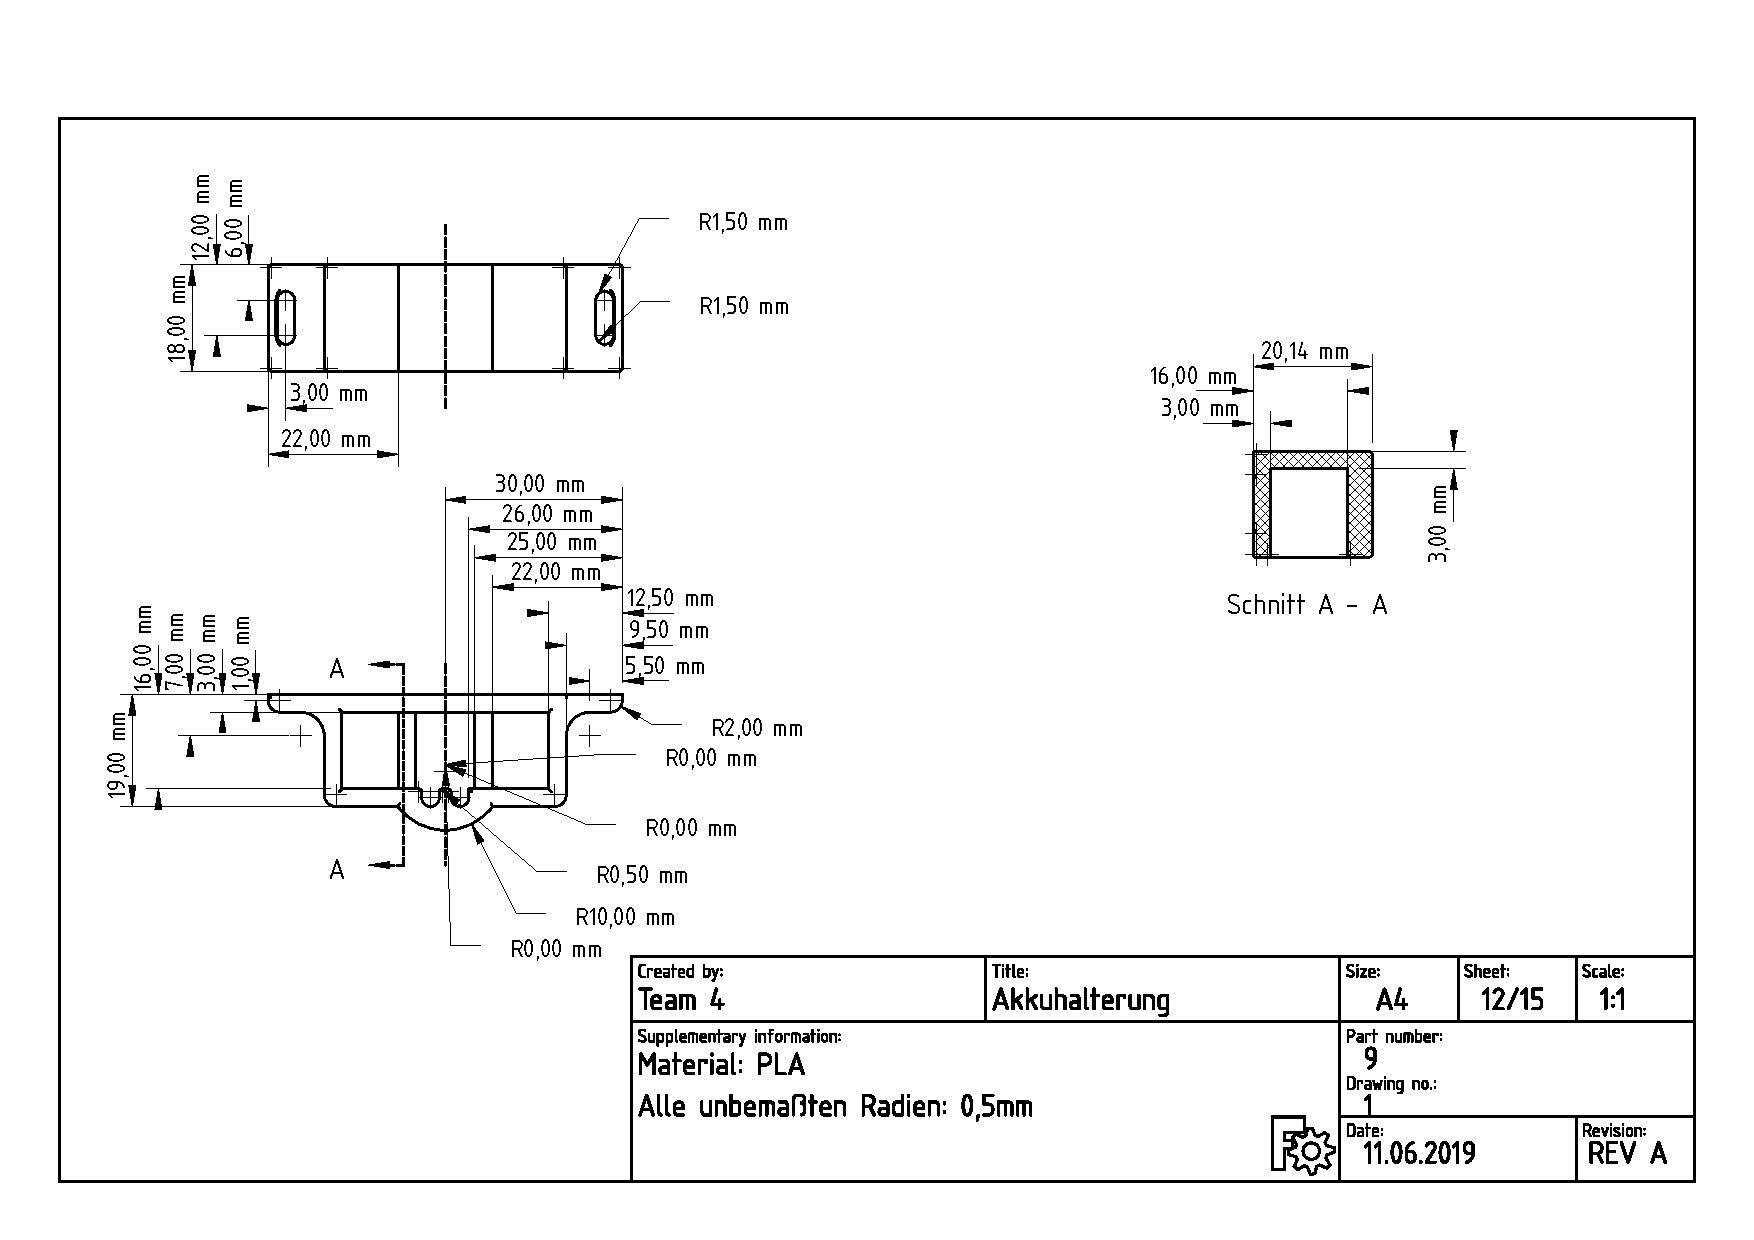
\includegraphics[width=\textwidth]{../techzeich/9.PDF} 	
	\caption{Akkuhalterung}
\end{figure}
\begin{figure}[ht!]
	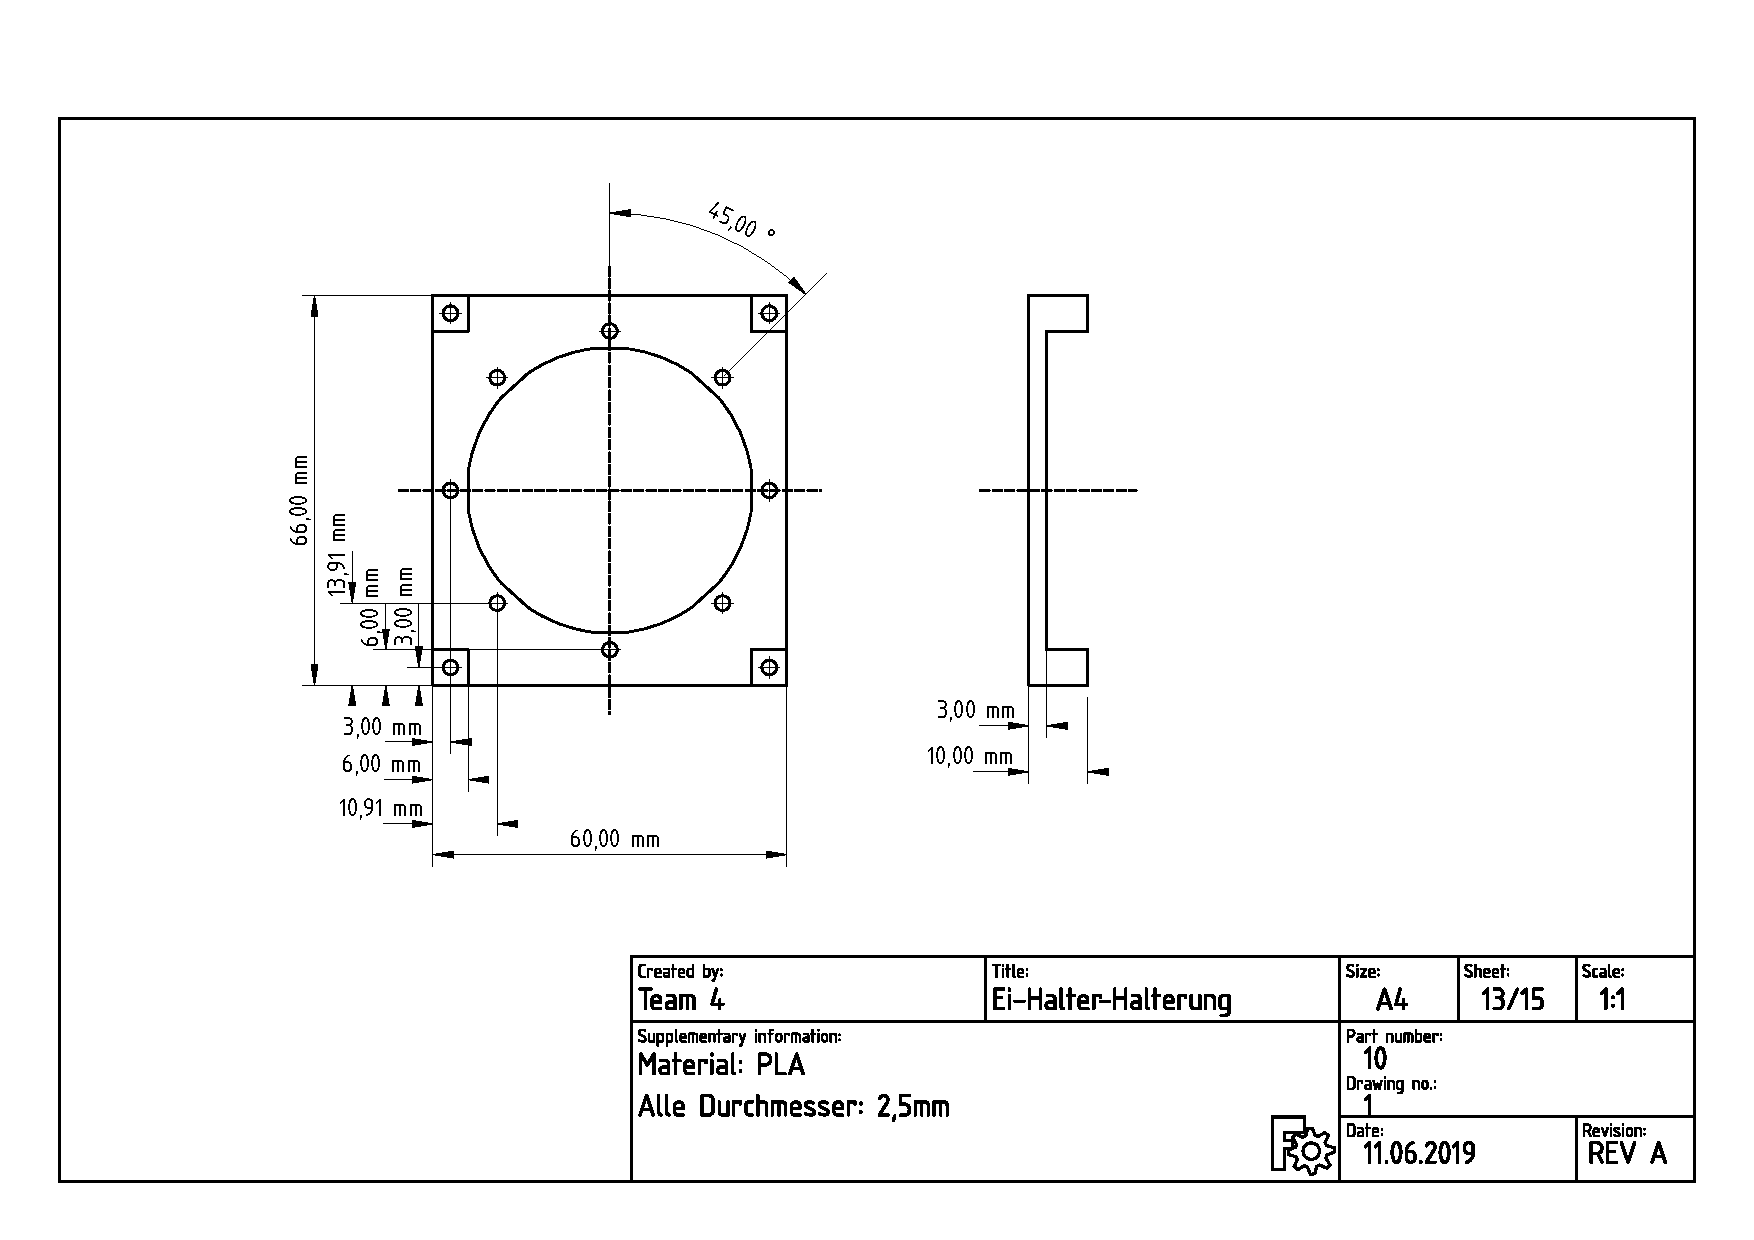
\includegraphics[width=\textwidth]{../techzeich/10.PDF} 	
	\caption{Ei-Halterung-Halterung}
\end{figure}
\begin{figure}[ht!]
	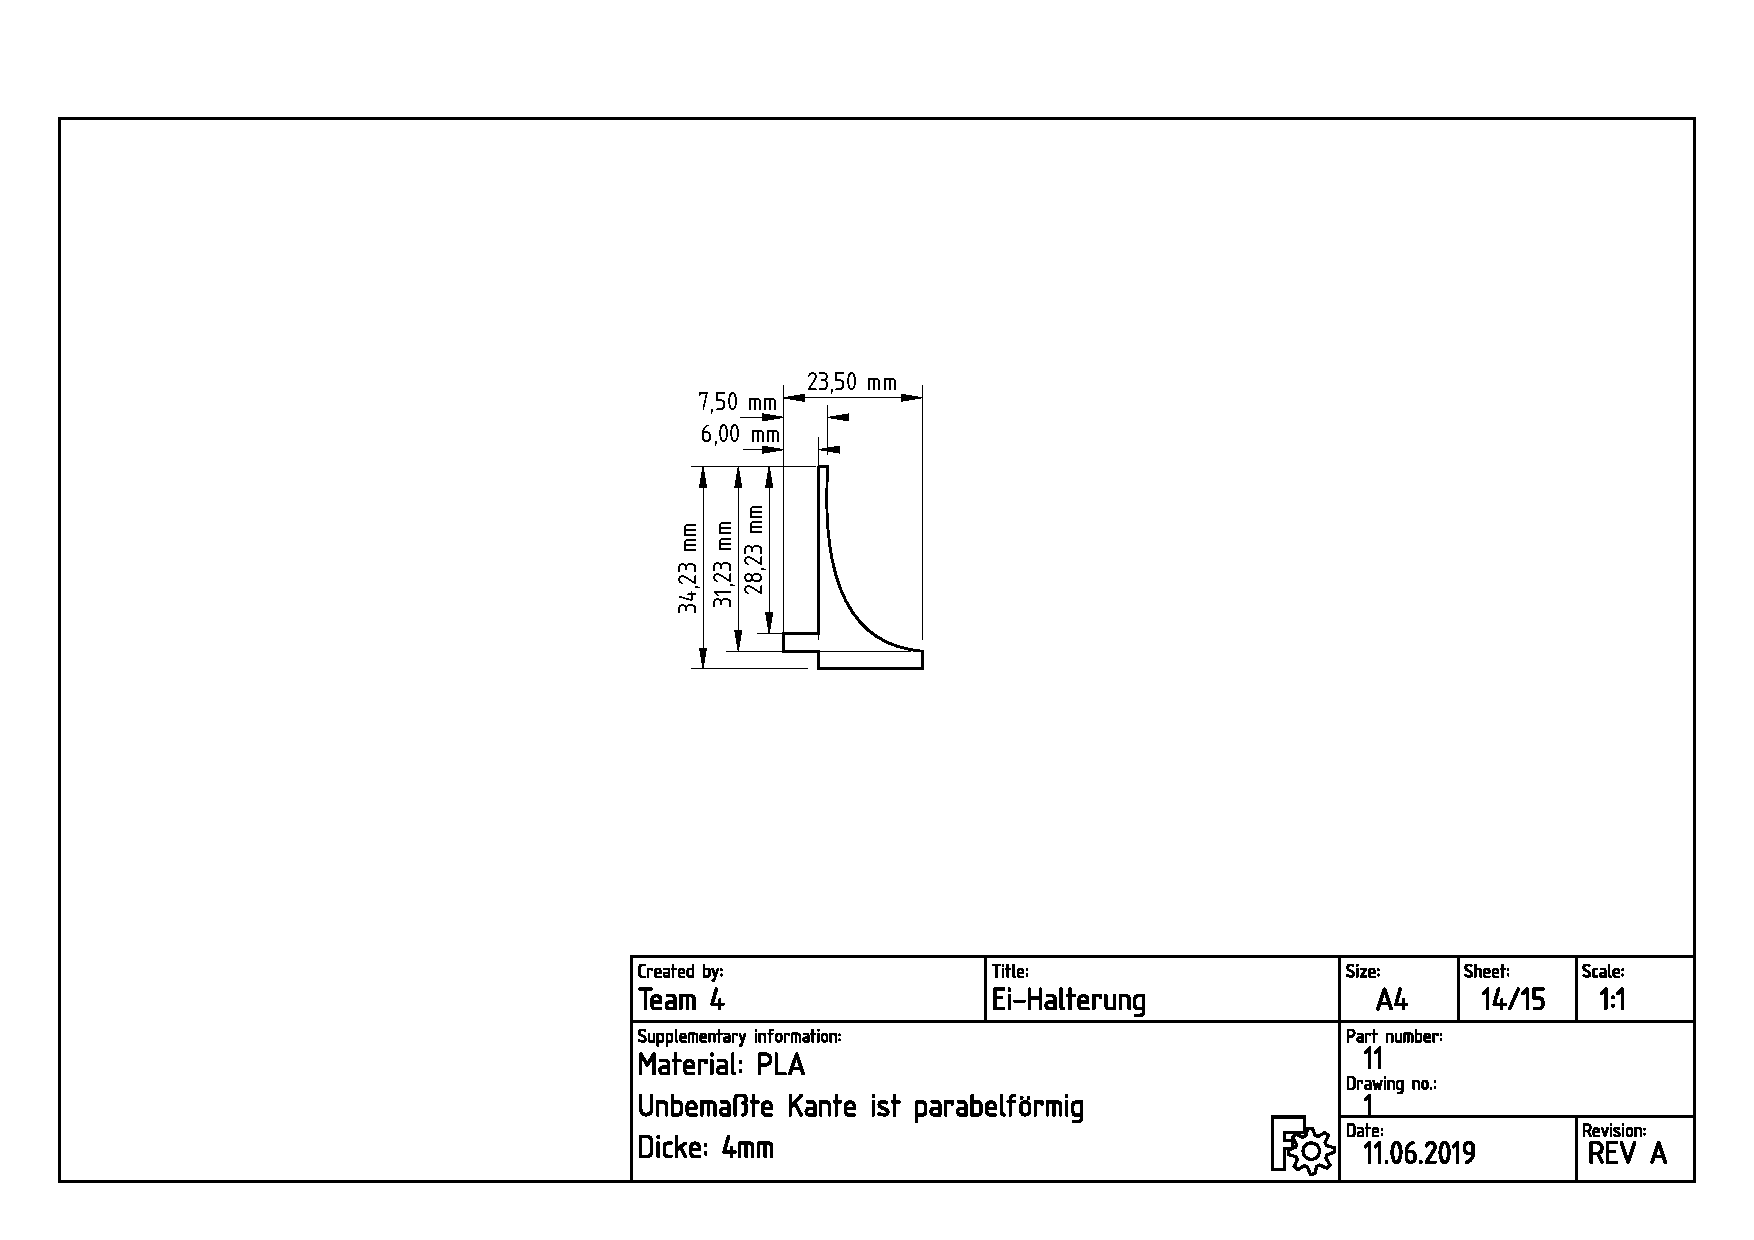
\includegraphics[width=\textwidth]{../techzeich/11.PDF} 	
	\caption{Ei-Halterung}
\end{figure}
\begin{figure}[ht!]
	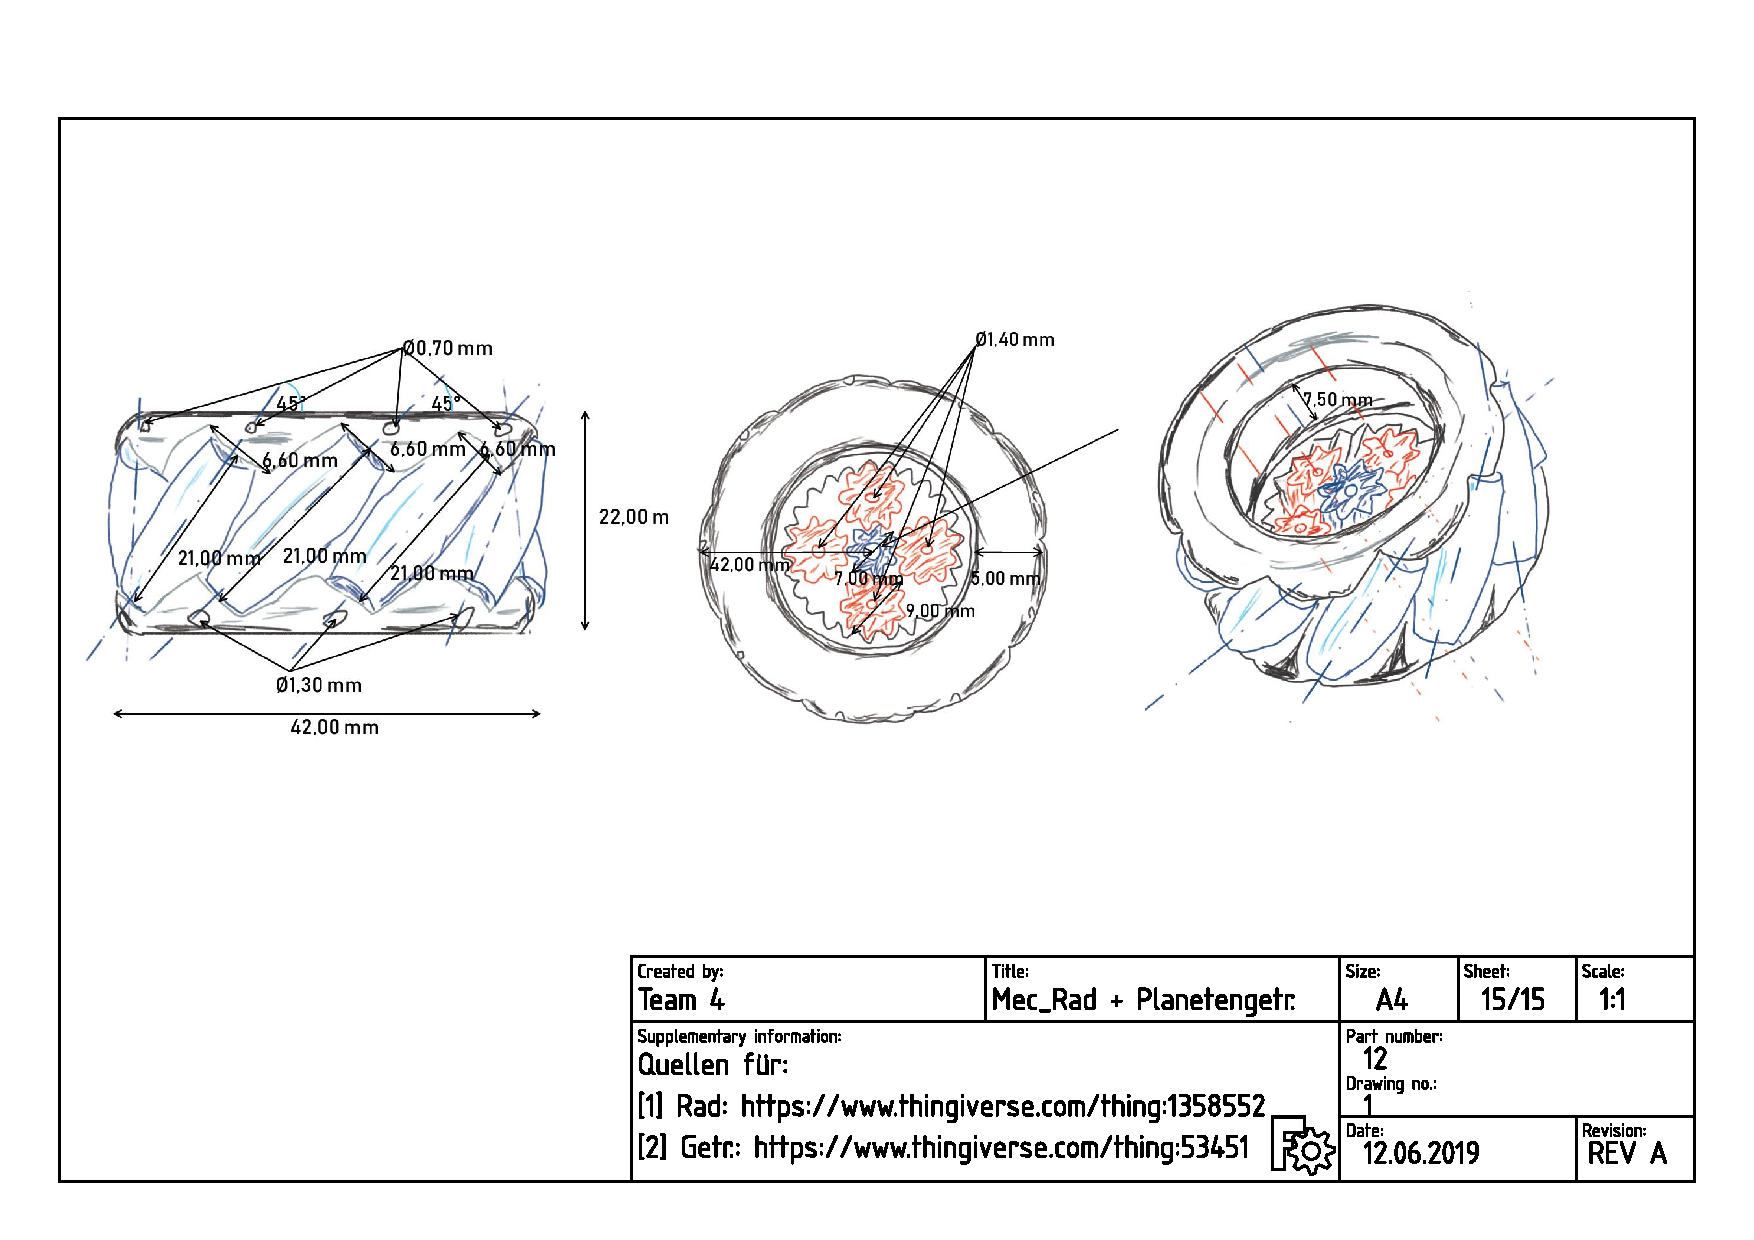
\includegraphics[width=\textwidth]{../techzeich/12.PDF} 	
	\caption{Reifen und Planetengetriebe}
\end{figure}